% !TeX spellcheck = en_US
% !TEX program = pdflatex
\documentclass[12pt,b5paper,notitlepage]{article}
\usepackage[b5paper, margin={0.5in,0.65in}]{geometry}
%\usepackage{fullpage}
\usepackage{mathtools} % perfect math mode, but seems not well for underbrace. It is recommended to use \begingroup in the file.
\let\underbrace\overbrace\relax
\usepackage{amsmath,amscd,amssymb,amsthm,mathrsfs,amsfonts,layout,indentfirst,graphicx,caption,mathabx, stmaryrd,appendix,calc,imakeidx,upgreek,amsbsy,thmtools} % mathabx for \wtidecheck
%\usepackage{ulem} %wave underline
\usepackage[dvipsnames]{xcolor}
\usepackage{palatino}  %template

\usepackage{stmaryrd}


\usepackage{slashed} % Dirac operator
\usepackage{mathrsfs} % Enable using \mathscr
%\usepackage{eufrak}  another template/font
\usepackage{extarrows} % long equal sign, \xlongequal{blablabla}
% \usepackage{pdfMsym}
\usepackage{enumitem} % enumerate label change e.g. [label=(\alph*)]  shows (a) (b) 

\usepackage{comment} % hide something


% \usepackage{titlesec}
% \usepackage{etoolbox}
% \pretocmd{\section}{\refstepcounter{section}\label{sec:\thesection}}{}{}
% \AtBeginEnvironment{theorem}{%
% 	\refstepcounter{theorem}%
% 	\edef\theoremname{\theoremname}% 获取定理的名字(如果有的话)
% 	\@ifundefined{theoremname}
%     {% 如果没有名字,只使用编号
%      \label{thm:\thesection.\thetheorem}%
%     }
%     {% 如果有名字,标签包含编号和名字
%      \label{thm:\thesection.\thetheorem.\theoremname}%
%     }
% }

%%%%%%%%%%%%%%%%%%%%%%%%%%%%%%

%\usepackage{fontspec}
%\setmainfont{Palatino Linotype}
%\usepackage{emoji}


% emoji, use lualatex  remove \usepackage{palatino}

%%%%%%%%%%%%%


\usepackage{CJK}   % Chinese package
\usepackage{pifont}




\usepackage{csquotes} % \begin{displayquote}   \begin{displaycquote}  for quotation
\usepackage{epigraph}   %\epigraph{}{}  for quotation
%\pmb  mandatory math bold 

\usepackage{fancyhdr} % date in footer



% 设置章节标题格式
% \titleformat{\section}[hang]{\normalfont\huge\bfseries}{\thesection}{2pc}{}

% \pagestyle{fancy}
% \fancyhead[L]{\rightmark}  % 左侧显示章节名
% \fancyhead[C]{}           % 中间清空
% \fancyhead[R]{}           % 右侧清空
\pagestyle{plain}

%\usepackage{soul}  %\ul underline break line automatically

\usepackage{ulem}  % \uline  underline break line   also    \uwave

\usepackage{relsize} % use \mathlarger \larger \text{\larger[2]$...$} to enlarge the size of math symbols

\usepackage{verbatim}  % comment environment


\usepackage{halloweenmath} % Interesting halloween math symbols

%%%%%%%%%%%%%%%%%%%%%%%%%%%%%%
\usepackage{tcolorbox}
\tcbuselibrary{theorems}
% box around equations   \tcboxmath
%%%%%%%%%%%%%%%%%%%%%%%%%%%%%%%%%%




%%%%%%%%%%%%%%%%%%%%%%%%%%%%%
% circled colon and thick colon \hcolondel and \colondel

\usepackage{pdfrender}

\newcommand*{\hollowcolon}{%
	\textpdfrender{
		TextRenderingMode=Stroke,
		LineWidth=.1bp,
	}{:}%
}

\newcommand{\hcolondel}[1]{%
	\mathopen{\hollowcolon}#1\mathclose{\hollowcolon}%
}
\newcommand{\colondel}[1]{%
	\mathopen{:}#1\mathclose{:}%
}

%%%%%%%%%%%%%%%%%%%%%%%%%%%%%%%%


\usepackage{setspace}  
\setstretch{1.6}



\usepackage{tikz}
\usetikzlibrary{fadings}
\usetikzlibrary{patterns}
\usetikzlibrary{shadows.blur}
\usetikzlibrary{shapes}
% \usetikzlibrary{graphs,graphdrawing,circular}

% \usetikzlibrary{graphs, graphdrawing, shapes.geometric, arrows}

\usepackage{tikz-cd}
\usepackage[nottoc]{tocbibind}   % Add  reference to ToC


\makeindex


% The following set up the line spaces between items in \thebibliography
\usepackage{lipsum}  
\let\OLDthebibliography\thebibliography
\renewcommand\thebibliography[1]{
	\OLDthebibliography{#1}
	\setlength{\parskip}{0pt}
	\setlength{\itemsep}{2pt} 
}


%\hyperref{page.10}{...}

\allowdisplaybreaks  %allow aligns to break between pages
\usepackage{latexsym}
\usepackage{chngcntr}
\usepackage[colorlinks,linkcolor=blue,anchorcolor=blue, linktocpage,
%pagebackref
]{hyperref}
\hypersetup{ urlcolor=cyan,
	citecolor=[rgb]{0,0.5,0}}


\setcounter{tocdepth}{2}	 %hide subsections in the content


\counterwithin{figure}{section}

\counterwithin*{footnote}{section}   % Footnote numbering is recounted from the beginning of each subsection




% \pagestyle{plain}

% \captionsetup[figure]
% {
% 	labelsep=none	
% }
% 控制图表结构











\theoremstyle{definition}
\newtheorem{definition}{Definition}[section]
\newtheorem{example}[definition]{Example}
\newtheorem{exercise}[definition]{Exercise}
\newtheorem{remark}[definition]{Remark}
\newtheorem{observation}[definition]{Observation}
\newtheorem{assumption}[definition]{Assumption}
\newtheorem{convention}[definition]{Convention}
\newtheorem{priniple}[definition]{Principle}
\newtheorem{notation}[definition]{Notation}
\newtheorem*{axiom}{Axiom}
\newtheorem{coa}[definition]{Theorem}
\newtheorem{srem}[definition]{$\star$ Remark}
\newtheorem{seg}[definition]{$\star$ Example}
\newtheorem{sexe}[definition]{$\star$ Exercise}
\newtheorem{sdf}[definition]{$\star$ Definition}
\newtheorem{question}{Question}
\theoremstyle{remark}
\newtheorem{note}{Note}
\theoremstyle{definition}
\newtheorem{claim}{Claim}[subsection]


\newtheorem{problem}{\color{red}Problem}[section]
%\renewcommand*{\theprob}{{\color{red}\arabic{section}.\arabic{prob}}}
\newtheorem{sprob}[problem]{\color{red}$\star$ Problem}
%\renewcommand*{\thesprob}{{\color{red}\arabic{section}.\arabic{sprob}}}
% \newtheorem{ssprob}[prob]{$\star\star$ Problem}



\theoremstyle{plain}
\newtheorem{theorem}[definition]{Theorem}
\newtheorem{Conclusion}[definition]{Conclusion}
\newtheorem{thd}[definition]{Theorem-Definition}
\newtheorem{proposition}[definition]{Proposition}
\newtheorem{corollary}[definition]{Corollary}
\newtheorem{lemma}[definition]{Lemma}
\newtheorem{sthm}[definition]{$\star$ Theorem}
\newtheorem{slm}[definition]{$\star$ Lemma}

\newtheorem{spp}[definition]{$\star$ Proposition}
\newtheorem{scorollary}[definition]{$\star$ Corollary}
\newtheorem{fact}[definition]{Fact}

\newtheorem{cond}{Condition}
\newtheorem{Mthm}{Main Theorem}
\renewcommand{\thecond}{\Alph{cond}} % "letter-numbered" theorems
\renewcommand{\theMthm}{\Alph{Mthm}} % "letter-numbered" theorems


%\substack   multiple lines under sum
%\underset{b}{a}   b is under a


% Remind: \overline{L_0}



\usepackage{calligra}
\DeclareMathOperator{\shom}{\mathscr{H}\text{\kern -3pt {\calligra\large om}}\,}
\DeclareMathOperator{\sext}{\mathscr{E}\text{\kern -3pt {\calligra\large xt}}\,}
\DeclareMathOperator{\Rel}{\mathscr{R}\text{\kern -3pt {\calligra\large el}~}\,}
\DeclareMathOperator{\sann}{\mathscr{A}\text{\kern -3pt {\calligra\large nn}}\,}
\DeclareMathOperator{\send}{\mathscr{E}\text{\kern -3pt {\calligra\large nd}}\,}
\DeclareMathOperator{\stor}{\mathscr{T}\text{\kern -3pt {\calligra\large or}}\,}
%write mathscr Hom (and so on) 

\usepackage{aurical}
\DeclareMathOperator{\VVir}{\text{\Fontlukas V}\text{\kern -0pt {\Fontlukas\large ir}}\,}

\newcommand{\vol}{\text{\Fontlukas V}}
\newcommand{\dvol}{d~\text{\Fontlukas V}}
% perfect Vol symbol

\usepackage{aurical}
\usepackage[T1]{fontenc}








\newcommand{\fk}{\mathfrak}
\newcommand{\mc}{\mathcal}
\newcommand{\wtd}{\widetilde}
\newcommand{\wht}{\widehat}
\newcommand{\wch}{\widecheck}
\newcommand{\ovl}{\overline}
\newcommand{\udl}{\underline}
\newcommand{\tr}{\mathrm{tr}} %transpose
\newcommand{\Tr}{\mathrm{T}}
\newcommand{\End}{\mathrm{End}} %endomorphism
\newcommand{\idt}{\mathbf{1}}
\newcommand{\id}{\mathrm{id}}
\newcommand{\Hom}{\mathrm{Hom}}
\newcommand{\Conf}{\mathrm{Conf}}
\newcommand{\Res}{\mathrm{Res}}
\newcommand{\res}{\mathrm{res}}
\newcommand{\KZ}{\mathrm{KZ}}
\newcommand{\ev}{\mathrm{ev}}
\newcommand{\coev}{\mathrm{coev}}
\newcommand{\opp}{\mathrm{opp}}
\newcommand{\Rep}{\mathrm{Rep}}
\newcommand{\diag}{\mathrm{diag}}
\newcommand{\Dom}{\mathrm{Dom}}
\newcommand{\loc}{\mathrm{loc}}
\newcommand{\con}{\mathrm{c}}
\newcommand{\uni}{\mathrm{u}}
\newcommand{\ssp}{\mathrm{ss}}
\newcommand{\di}{\slashed d}
\newcommand{\Diffp}{\mathrm{Diff}^+}
\newcommand{\Diff}{\mathrm{Diff}}
\newcommand{\PSU}{\mathrm{PSU}(1,1)}
\newcommand{\Vir}{\mathrm{Vir}}
\newcommand{\Witt}{\mathscr W}
\newcommand{\Span}{\mathrm{Span}}
\newcommand{\pri}{\mathrm{p}}
\newcommand{\ER}{E^1(V)_{\mathbb R}}
\newcommand{\prth}[1]{( {#1})}
\newcommand{\bk}[1]{\langle {#1}\rangle}
\newcommand{\bigbk}[1]{\big\langle {#1}\big\rangle}
\newcommand{\Bigbk}[1]{\Big\langle {#1}\Big\rangle}
\newcommand{\biggbk}[1]{\bigg\langle {#1}\bigg\rangle}
\newcommand{\Biggbk}[1]{\Bigg\langle {#1}\Bigg\rangle}
\newcommand{\GA}{\mathscr G_{\mathcal A}}
\newcommand{\vs}{\varsigma}
\newcommand{\Vect}{\mathrm{Vec}}
\newcommand{\Vectc}{\mathrm{Vec}^{\mathbb C}}
\newcommand{\scr}{\mathscr}
\newcommand{\sjs}{\subset\joinrel\subset}
\newcommand{\Jtd}{\widetilde{\mathcal J}}
\newcommand{\gk}{\mathfrak g}
\newcommand{\hk}{\mathfrak h}
\newcommand{\xk}{\mathfrak x}
\newcommand{\yk}{\mathfrak y}
\newcommand{\zk}{\mathfrak z}
\newcommand{\pk}{\mathfrak p}
\newcommand{\hr}{\mathfrak h_{\mathbb R}}
\newcommand{\Ad}{\mathrm{Ad}}
\newcommand{\DHR}{\mathrm{DHR}_{I_0}}
\newcommand{\Repi}{\mathrm{Rep}_{\wtd I_0}}
\newcommand{\im}{\mathbf{i}}
\newcommand{\Co}{\complement}
%\newcommand{\Cu}{\mathcal C^{\mathrm u}}
\newcommand{\RepV}{\mathrm{Rep}^\uni(V)}
\newcommand{\RepA}{\mathrm{Rep}(\mathcal A)}
\newcommand{\RepN}{\mathrm{Rep}(\mathcal N)}
\newcommand{\RepfA}{\mathrm{Rep}^{\mathrm f}(\mathcal A)}
\newcommand{\RepAU}{\mathrm{Rep}^\uni(A_U)}
\newcommand{\RepU}{\mathrm{Rep}^\uni(U)}
\newcommand{\RepL}{\mathrm{Rep}^{\mathrm{L}}}
\newcommand{\HomL}{\mathrm{Hom}^{\mathrm{L}}}
\newcommand{\EndL}{\mathrm{End}^{\mathrm{L}}}
\newcommand{\Bim}{\mathrm{Bim}}
\newcommand{\BimA}{\mathrm{Bim}^\uni(A)}
%\newcommand{\shom}{\scr Hom}
\newcommand{\divi}{\mathrm{div}}
\newcommand{\sgm}{\varsigma}
\newcommand{\SX}{{S_{\fk X}}}
\newcommand{\DX}{D_{\fk X}}
\newcommand{\mbb}{\mathbb}
\newcommand{\mbf}{\mathbf}
\newcommand{\bsb}{\boldsymbol}
\newcommand{\blt}{\bullet}
\newcommand{\Vbb}{\mathbb V}
\newcommand{\Ubb}{\mathbb U}
\newcommand{\Xbb}{\mathbb X}
\newcommand{\Kbb}{\mathbb K}
\newcommand{\Abb}{\mathbb A}
\newcommand{\Wbb}{\mathbb W}
\newcommand{\Mbb}{\mathbb M}
\newcommand{\Gbb}{\mathbb G}
\newcommand{\Cbb}{\mathbb C}
\newcommand{\Nbb}{\mathbb N}
\newcommand{\Zbb}{\mathbb Z}
\newcommand{\Qbb}{\mathbb Q}
\newcommand{\Pbb}{\mathbb P}
\newcommand{\Rbb}{\mathbb R}
\newcommand{\Ebb}{\mathbb E}
\newcommand{\Dbb}{\mathbb D}
\newcommand{\Hbb}{\mathbb H}
\newcommand{\cbf}{\mathbf c}
\newcommand{\Rbf}{\mathbf R}
\newcommand{\wt}{\mathrm{wt}}
\newcommand{\Lie}{\mathrm{Lie}}
\newcommand{\btl}{\blacktriangleleft}
\newcommand{\btr}{\blacktriangleright}
\newcommand{\svir}{\mathcal V\!\mathit{ir}}
\newcommand{\Ker}{\mathrm{Ker}}
\newcommand{\Cok}{\mathrm{Coker}}
\newcommand{\Sbf}{\mathbf{S}}
\newcommand{\low}{\mathrm{low}}
\newcommand{\Sp}{\mathrm{Sp}}
\newcommand{\Rng}{\mathrm{Rng}}
\newcommand{\vN}{\mathrm{vN}}
\newcommand{\Ebf}{\mathbf E}
\newcommand{\Nbf}{\mathbf N}
\newcommand{\Stb}{\mathrm {Stb}}
\newcommand{\SXb}{{S_{\fk X_b}}}
\newcommand{\pr}{\mathrm {pr}}
\newcommand{\SXtd}{S_{\wtd{\fk X}}}
\newcommand{\univ}{\mathrm {univ}}
\newcommand{\vbf}{\mathbf v}
\newcommand{\ubf}{\mathbf u}
\newcommand{\wbf}{\mathbf w}
\newcommand{\CB}{\mathrm{CB}}
\newcommand{\Perm}{\mathrm{Perm}}
\newcommand{\Orb}{\mathrm{Orb}}
\newcommand{\Lss}{{L_{0,\mathrm{s}}}}
\newcommand{\Lni}{{L_{0,\mathrm{n}}}}
\newcommand{\UPSU}{\widetilde{\mathrm{PSU}}(1,1)}
\newcommand{\Sbb}{{\mathbb S}}
\newcommand{\Gc}{\mathscr G_c}
\newcommand{\Obj}{\mathrm{Obj}}
\newcommand{\bpr}{{}^\backprime}
\newcommand{\fin}{\mathrm{fin}}
\newcommand{\Ann}{\mathrm{Ann}}
\newcommand{\Real}{\mathrm{Re}}
\newcommand{\Imag}{\mathrm{Im}}
%\newcommand{\cl}{\mathrm{cl}}
\newcommand{\Ind}{\mathrm{Ind}}
\newcommand{\Supp}{\mathrm{Supp}}
\newcommand{\Specan}{\mathrm{Specan}}
\newcommand{\red}{\mathrm{red}}
\newcommand{\uph}{\upharpoonright}
\newcommand{\Mor}{\mathrm{Mor}}
\newcommand{\pre}{\mathrm{pre}}
\newcommand{\rank}{\mathrm{rank}}
\newcommand{\Jac}{\mathrm{Jac}}
\newcommand{\emb}{\mathrm{emb}}
\newcommand{\Sg}{\mathrm{Sg}}
\newcommand{\Nzd}{\mathrm{Nzd}}
\newcommand{\Owht}{\widehat{\scr O}}
\newcommand{\Ext}{\mathrm{Ext}}
\newcommand{\Tor}{\mathrm{Tor}}
\newcommand{\Com}{\mathrm{Com}}
\newcommand{\Mod}{\mathrm{Mod}}
\newcommand{\nk}{\mathfrak n}
\newcommand{\mk}{\mathfrak m}
\newcommand{\Ass}{\mathrm{Ass}}
\newcommand{\depth}{\mathrm{depth}}
\newcommand{\Coh}{\mathrm{Coh}}
\newcommand{\Gode}{\mathrm{Gode}}
\newcommand{\Fbb}{\mathbb F}
\newcommand{\sgn}{\mathrm{sgn}}
\newcommand{\Aut}{\mathrm{Aut}}
\newcommand{\Modf}{\mathrm{Mod}^{\mathrm f}}
\newcommand{\codim}{\mathrm{codim}}
\newcommand{\card}{\mathrm{card}}
\newcommand{\dps}{\displaystyle}
\newcommand{\Int}{\mathrm{Int}}
\newcommand{\Nbh}{\mathrm{Nbh}}
\newcommand{\Pnbh}{\mathrm{PNbh}}
\newcommand{\Cl}{\mathrm{Cl}}
\newcommand{\diam}{\mathrm{diam}}
\newcommand{\eps}{\varepsilon}
\newcommand{\Vol}{\mathrm{Vol}}
\newcommand{\LSC}{\mathrm{LSC}}
\newcommand{\USC}{\mathrm{USC}}
\newcommand{\Ess}{\mathrm{Rng}^{\mathrm{ess}}}
\newcommand{\Jbf}{\mathbf{J}}
\newcommand{\SL}{\mathrm{SL}}
\newcommand{\GL}{\mathrm{GL}}
\newcommand{\Lin}{\mathrm{Lin}}
\newcommand{\ALin}{\mathrm{ALin}}
\newcommand{\bwn}{\bigwedge\nolimits}
\newcommand{\nbf}{\mathbf n}
\newcommand{\dive}{\mathrm{div}}
\newcommand{\Alt}{\mathrm{Alt}}
\newcommand{\Sym}{\mathrm{Sym}}



\renewcommand{\epsilon}{\varepsilon}
% \renewcommand{\phi}{\varphi}





\usepackage{tipa} % wierd symboles e.g. \textturnh
\newcommand{\tipar}{\text{\textrtailr}}
\newcommand{\tipaz}{\text{\textctyogh}}
\newcommand{\tipaomega}{\text{\textcloseomega}}
\newcommand{\tipae}{\text{\textrhookschwa}}
\newcommand{\tipaee}{\text{\textreve}}
\newcommand{\tipak}{\text{\texthtk}}
\newcommand{\mol}{\upmu}
\newcommand{\dmol}{d\upmu}




\usepackage{tipx}
\newcommand{\tipxgamma}{\text{\textfrtailgamma}}
\newcommand{\tipxcc}{\text{\textctstretchc}}
\newcommand{\tipxphi}{\text{\textqplig}}















\numberwithin{equation}{section}
% count the eqation by section countation



\title{Discrete Optimization}
\author{
	{{\bf Instructor:} Yuan Zhou}\\
	{{\bf Notes Taker:} Zejin Lin}\\
	{\small \sc Tsinghua University.}\\
	{\small linzj23@mails.tsinghua.edu.cn}\\
	{\small \href{lzjmaths.github.io}{lzjmaths.github.io}}
}

\DeclareMathOperator{\sign}{sign}
\DeclareMathOperator{\dom}{dom}
\DeclareMathOperator{\ran}{ran}
\DeclareMathOperator{\ord}{ord}
\DeclareMathOperator{\img}{Im}
\DeclareMathOperator{\argmin}{argmin}
\DeclareMathOperator{\argmax}{argmax}
\newcommand{\OPT}{\mathrm{OPT}}
\newcommand{\dd}{\mathrm{d}}
\newcommand{\ie}{ \textit{ i.e. } }
\newcommand{\st}{ \textit{ s.t. }}
\newcommand{\name}[1]{\textbf{#1}\index{#1}}
\newcommand{\subname}[2]{\textbf{#1}\index{#2!#1}}
\newcommand{\stdO}{\mathcal{O}_{\mathrm{std}}}
\newcommand{\stdwedge}[1]{\dd {#1}^1\wedge\cdots\wedge\dd {#1}^n}
\newcommand{\stddownwedge}[1]{\dd {#1}_1\wedge\cdots\wedge\dd {#1}_n}

\newcommand{\opensub}{\overset{\text{open}}{\subset}}
\newcommand{\chart}[2]{({#1}_\alpha,{#2}^1,\cdots,{#2}^n)}
\newcommand{\<}{\left<}
\renewcommand{\>}{\right>}
\renewcommand{\|}{\Vert}
\renewcommand{\hat}[1]{\widehat{#1}}
\renewcommand{\tilde}[1]{\widetilde{#1}}
\newcommand{\Romannumer}[1]{\mathrm{\uppercase\expandafter{\romannumeral#1}}}
\newcommand{\rot}{\mathrm{rot}}

\renewcommand{\div}{\mathrm{div}}
%\makeindex[columns=2,title=Index, options=-s example_style.ist]
\usepackage{pgfplots}
\pgfplotsset{width=7cm,compat=1.18}
\usepackage{algorithm}
\usepackage{algorithmic}

\usepackage{chemarrow}

% \usepackage{tikz-3dplot} 
% \renewcommand{\xrightarrow}[2]{\autorightarrow{#1}{#2}}

% \excludecomment{proof}
% \excludecomment{remark}
% \excludecomment{definition}
% \excludecomment{example}
% \excludecomment{exercise}

\tikzset{
  curarrow/.style={
  rounded corners=8pt,
  execute at begin to={every node/.style={fill=red}},
    to path={-- ([xshift=-50pt]\tikztostart.center)
    |- (#1) node[fill=white] {$\scriptstyle d$}
    -| ([xshift=50pt]\tikztotarget.center)
    -- (\tikztotarget)}
    }
}

\begin{document}
\sloppy
\pagenumbering{arabic}
\maketitle
\tableofcontents
\newpage

\section{Regression}
\begin{equation}\label{Lasso}
    \min_{\omega\in \Rbb^m}\frac{1}{2N}\|\Phi\omega-y\|^2+\lambda C(\omega)
\end{equation}

\name{Lasso}:  $ C=\|\omega\|_1 $. \name{Ridge regression}: $ C=\|\omega\|_2 $.

\name{subgradient} of  $ f $:
\[\partial f(x_0)=\{g|f(x) \geq f(x_0)+g^T(x-x_0)\}\] 
In particular, 
\[\partial |x|=\begin{cases}
    1, & x>0\\
    -1, & x<0\\
    [-1,1], & x=0
\end{cases}\]

\subsection{Binary classification problem}
\name{one-hot encoding} for the output  $ \{\binom{1}{0},\binom{0}{1} \} $. It can be understood as the probability for each class  and can take continuous values.

A \name{linear hypothesis space} is  $ \{u(x):u=\omega^Tx,x\in \Rbb^n,\omega\in \Rbb^n\} $.

\name{Softmax}:Map the extracted feature  $ u $ to the space of one-hot codes 
\[\mu=\frac{1}{1+e^{-u}},\quad 1-\mu=\frac{e^{-u}}{1+e^{-u}}=\frac{1}{1+e^{u}}\] 

\begin{equation}\label{KL distance}
    KL(p,q)=\int p(\log p - \log q)
\end{equation}
For  $ p $ real probability, to minimize \eqref{KL distance}, suffices to minimize 
\[-\int p\log q_\theta\dd x=-\sum_{x_i}\log q_\theta(x_i)\] 
which is called \name{Maximum likelihood} (\name{cross entropy})
\[-\sum \log p(y_i|x_i,\omega)=\sum -y_i\log \mu_i-(1-y_i)\log (1-\mu_i)\]
We reduce to minimize the thing above.

\subsection{Gradient Descent}
\[J(\theta)=\sum_{i=1}^N L(f_\theta(x_i),y_i),\quad \theta^{t+1}=\theta^t-\eta_t\frac{\partial J(\theta)}{\partial \theta}|_{\theta=\theta^t}\]

%!TEX root = /lecture/Discrete_Optimistic.tex

\subsection{Single-Source Shortest Path}
\begin{example}[Single-Source Shortest Path(SSSP)]
    Input: Graph $ G=(V,E,w) $,  $ V $ is the set of point and  $ E $ is the set of edge with direction  and  $ \omega:E\rightarrow \Rbb_{ \geq 0} $.
    
    We want to find a path from  $ s $ to  $ t $ with minimum total cost.
\end{example}
\paragraph{Dijkstra's Algorithm}
Choose  $ s  $ as a source.  $ d[s]=0,d[u]=\begin{cases}
    \omega(s,u)&\text{if  $ (s,u)\in E $}\\
    +\infty &\text{otherwise}
\end{cases} $, $ S=\{s\} $ first. To record the path, we can use  $ \mathrm{Pred}[u]\leftarrow s $.  

\begin{algorithm}
    \caption{Dijkstra's Algorithm}
    \label{alg:dijkstra}
    \begin{algorithmic}[1]
    \WHILE{$ S\neq V $}
        \STATE Choose  $ u\in \dps\arg\min_{\not\in S}\{d[x]\} $.\label{Choose u min}
        \STATE Update  $ S\leftarrow S\cup\{u\} $.
        \FOR{each $ x\in V-S $,$ (u,x)\in E $}
            \STATE$ d[x]\leftarrow\min\{d[x],d[u]+\omega(u,x)\} $.
            \IF{ $ d[u]+\omega(u,x)<d[x] $ }
                \STATE  $ d[x]\leftarrow d[u]+\omega(u,x) $  
                \STATE  $ \mathrm{Pred}[x]\leftarrow u $  
            \ENDIF
        \ENDFOR 
    \ENDWHILE
    \end{algorithmic}
\end{algorithm}

\begin{theorem}[Invariant]
    $ \forall u\in S $, $ d[u] $ is the shortest path distance  $ s\leadsto u $   
\end{theorem}
\begin{proof}
    Induction on  $ |S| $.
    
    For  $ |S|=1 $ true.

    \textbf{Induction Step: } Every time executing \ref{Choose u min} in Algorithm \ref{alg:dijkstra}, we need to prove  $ d[u] $ is the shortest distance  $ s\leadsto u $.

    If  $ v=\mathrm{Pred}[u]\in S $, then  $ d[u]=d[v]+\omega(v,u) $.
    
    For any path from  $ s $  to  $ u $, there exists  $ (\alpha,\beta)\in E $ such that  $ \alpha\in S,\beta\not\in S $. Then 
    \begin{align*}
        \mathrm{length}(P)& \geq \mathrm{length}(P[s\rightarrow\beta])\\
        & =\mathrm{length}(P[s\rightarrow\alpha])+\omega(\alpha,\beta)\\
        & \geq d[\alpha]+\omega(\alpha,\beta)\\
        & \geq d[\beta] \geq d[u]
    \end{align*}   
\end{proof}

\begin{remark}
    The straightforward implementation of Dijkstra's Algorithm is of  $ O(|v|^2) $.
    
    If we use priority queue: $ Q $ with priority  $ Q.\pi() $. It has some methods:
    \begin{itemize}
        \item ExtractMin: Return  $ \dps\arg\min_{x\in Q}\{Q.\pi(x)\} $ and remove  $ x  $ from  $ Q $.
        \item DecreaseKey: Update  $ Q.\pi(v) $ with newkey. 
    \end{itemize}  
    The time complexity is  $ |V|\times $ ExtractMin  $ + $ $ |E|\times  $  DecreaseKey    
    \begin{center}
        \begin{tabular}{|c|c|c|c|}
            \hline
            Runtime & ExtractMin & DecreaseKey & Dijkstra\\ \hline
            Simple Array   &  $ O(|V|) $   &  $ O(1) $ & $ O(|v|^2) $    \\ \hline
            Binary Heap   &  $ O(\log|V|) $    &  $ O(\log |V|) $ & $ O(|E|\cdot \log|V|) $   \\ \hline
            Fibonacci Heap & $ O(\log|V|) $ &  $ O(1) $ (amorized)&   $ O(|E|+|V|\log|V|) $ \\ \hline
        \end{tabular}
    \end{center}
\end{remark}
\subsection{Minimum Spanning Tree}
\begin{example}[Minimum Spanning Tree (MST)]
    Input: Connected, undirected graph $ G=(V,E,\omega) $.
    
    \begin{definition}[Spanning Tree]
        $ T\subset E $ is a \name{spanning tree}  if  $ |T|=|V|-1 $,  $ G'=(V,T) $ is connected.
        
        \textbf{Goal of MST } Find spanning tree  $ T $ so that  $ \dps\omega(T)=\sum_{e\in T}\omega(e) $ minimized.  
    \end{definition}
    \begin{theorem}[Cayley Theorem]
        The number of spanning trees of  $ n $-vertex complete graph is  $ n^{n-2} $  
    \end{theorem}
    A \name{cut}  $ (S,V-S) $ has a \name{cutset} of  $ S $ $ =\{e=(u,v):u\in S,v\not\in S\} $.  
\end{example}

For \textbf{empirical loss} 
\[J(\theta)=\frac{1}{N}\sum_{i=1}^N J_i(\theta),J_i(\theta)L(f_\theta(y_i),x_i)\]
\name{Stochastic Gradient Descent}:only compute gradients over a mini batch for each epoch
\[\theta_{k+1}=\theta_k-\eta\frac{1}{B}\sum_{i\in I_B} \nabla  J_i(\theta_k)\]
$ I_B $, called \name{mini batch} are randomly sampled from the training data indexes.

The motivation to sample is that for distribution  $ x $,  $ \dps\frac{x_1+\cdots+x_N}{N} $ has the same mean  $ \mu  $ but less variance  $ \frac{1}{N}\sigma^2 $, so in order to have more randomness and greatly reduce the computational cost, we choose less ammount of data.

Randomness can help avoid getting stuck in  local minimum.

SGD: $ x_{t+1}=x_t-\alpha \nabla f(x_t) $.

SGD+\name{momentum}:
\[v_{t+1}=\rho v_t+\nabla f(X_t)\]
\[x_{t+1}=x_t-\alpha v_{t+1}\]
$ v_t $ is the momentum which helps accelerate convergence by accumulating the gradients of past steps and smoothing out the oscillations, where  $ \rho=0.9  $ or  $ 0.99 $.  

\subsection{Adaptive learning rate}

\[r_t=r_{t-1}+\nabla f(x_t)\bigodot  \nabla f(x_t)\]
\[x_{t+1}=x_t-\frac{\alpha}{\sqrt{r_t+\epsilon}}\bigodot  \nabla f(x_t)\]
For frequent features, the  updates will be smaller, and for rare features, the updates will be larger.

\paragraph{Notation}  $ \odot $ is  the multiplication for each component, which means:


\[\begin{pmatrix}
    a_1\\
    \vdots\\
    a_n
\end{pmatrix}\odot\begin{pmatrix}
    b_1\\
    \vdots\\
    b_n
\end{pmatrix}=\begin{pmatrix}
    a_1b_1\\
    \vdots\\
    a_nb_n
\end{pmatrix}\]

\section{MLP}

\name{Exponential Moving Averaging(EMA)}
\[r_t=\beta r_{t-1}+(1-\beta)\nabla f(x_t)\odot \nabla f(x_t)\]
\[x_{t+1}=x_t-\frac{\alpha}{\sqrt{r_t+\epsilon}}\bigodot  \nabla f(x_t)\]

RMSProp uses a moving average, avoiding overly aggresive decay complared with AdaGrad.

\name{Adaptive Moment Estimation(Adam)}:RMAProp+Momentum 
\[g_t=\nabla f(x_t)\]
\[v_t=\beta_1^t v_{t-1}+(1-\beta_1^t)g_t, r_t=\beta_2^t r_{t-1}+(1-\beta_2^t)g_t\odot g_t\]
\[v_t=\frac{v_t}{1-\beta_1^t},E_t=\frac{E_t}{1-\beta_2^t}\]
\[x_{t+1}=x_t-\frac{\alpha}{\sqrt{r_t+\epsilon}}\odot v_t\]

\section{Vanishing or Exploding Gradient}
The gradient of the Sigmoid function is very small most of the time, leading to vanishing gradients

We want to avoid exploding or vanishment in gradient.

\name{Sigmoid}: $ \dps\sigma(z)=\frac{1}{1+e^{-z}} $.

\name{Tanh}: $ \dps\sigma(z)=\frac{e^{z}-e^{-z}}{e^z+e^{-z}} $.

\name{ReLU}:  $ \dps\mathrm{ReLU}(z)=\begin{cases}
    z,&z>0\\
    0,&\text{otherwise}
\end{cases} $.

\name{LeakyReLU}: $ \dps \mathrm{LeakyReLU}(z)=\begin{cases}
    z,&z>0\\
    az,&\text{otherwise}
\end{cases} $.
The gradient neither vanishes nor explodes; it is computationally fast, but some neurons may not be activated.

LeakyReLU solves the issue with ReLU and is the most commonly used.

Consider the back propagation  $ \dps\frac{\partial J}{\partial x}=\frac{\partial J}{\partial y}\frac{\partial y}{\partial x}=\frac{\partial J}{\partial x}W$. Cumulate after multi-layers
\[\mathrm{Var}(\frac{\partial J}{\partial x})=\prod_i n_l \mathrm{Var}(W_l)\mathrm{Var}(\frac{\partial J}{\partial x_l})\]
We want   $ n_l\mathrm{Val}(W_l)\sim 1 $. 

After normalizing their variances, the updating becomes more steady and efficient.

To avoid variance becoming too small or too large in deep layers, normalize features in the network 
\[\hat{x}_i=\frac{x_i-\Ebb x_i}{\sqrt{\mathrm{var}(x_i)}}\]
\name{Batch Normalization}: normalize features across samples within each batch.





\begin{definition}
    Given directed  $ G=(V,E)  $ and  $ r\in V  $,  $ n=|V|,m=|E| $,  $ F\subset E $ is an \name{arborescence} if 
    \begin{itemize}
        \item  $ F $ is a spanning tree if ignoring directions
        \item   $ \forall v\in V $,  $ \exists $ unique  path  $ r\rightarrow v $ in  $ F $.    
    \end{itemize}  
    Or equivalently,  $ F $ has no directed cycles and every node  $ v\neg r $ has a unique incoming edge.  
\end{definition}

For this problem, WLOG we can assuem that the root  $ r $  has no in-degree and assume  $ \omega \geq 0 $.  

\newcommand{\cheap}{\mathrm{cheap}}
For each  $ n\neq r $, let 
\[\mathrm{cheap}(v)=\argmin_{e=(u,v)\in E}\{\omega(e)\}\] 
\begin{claim}
    Let  $ F=\{\cheap(v)|v\neq r\} $.  $ F $ is arborescense $ \Rightarrow  $  $ F $ is min-cost.   
\end{claim}

Define  $ \omega_r(u,v)=\omega(u,v)-\omega(\cheap(v)) $. Suffices to find the min-cost arborescence under  $ \omega_r $. 

If  $ F $ is not an arborescense, then  $ \exists $ a directed cycle  $ C $ with all edges of weight  $ 0 $.    


Using the contraction view, if we contract "$ 0 $-cycle" and keep this process recursively. By taking degrees carefully we can easily confirm the legallity of the contraction view. Then suffices to prove it is indeed the min-cost arborescence when we expand after.

\begin{theorem}
    The min-cost arborescence  $ \tilde{F} $ when we apply contraction to  $ 0- $cycle is exactly the min-cost arborescence in the original graph after expanding.  
\end{theorem}
\begin{lemma}
    $ \exists $ min-cost  $ F^* $ \st only 1 edge in  $ F^* $ entering  $ C $.   
\end{lemma}
\begin{proof}
    Our goal is to prove  $ \omega_r(F) \leq \omega_r(F^*) $. 

    Let  $ F^*_C=F^*\cap (C\times C) $. Then  $ |F^*_C|=|C|-1 $.
    
    Apply  $ C $-contraction to  $ F^*\setminus F^*_C $ we obtain an arborescence of  $ \tilde{G} $. (Easy to check) So 
    \[\sum_{e\in F^*\setminus F^*_C}\omega_r(e) \geq \sum_{e\in \tilde{F}}\omega_r(e)\]
    So  $ \omega_r(F^*) \geq \omega_r(F) $ 
\end{proof}
\begin{proof}[Proof of Lemma]
    Choose any  $ v\in C $.
    
    Let  $ (x,y)\in r\rightarrow v $ be the first edge entering  $ C $.
    
    Delete the edge entering  $ C\setminus\{y\} $ and add the edge of circle  except the edge entering  $ y $.
    
    Then it is  an arborescence of less cost.
\end{proof}
\section{Dynamic Programming}
\subsection{Weighted Interval Scheduling}
\begin{example}[Weighted Interval Scheduling]
    Input: $ n $ jobs,  $ \{(s_i,f_i),\omega_i\}_{i=1}^n $. Want to find  $ \sum\omega_{i_k} $ maximum.  
\end{example}

To make the structure simpler, we WLOG assume  $ s_1 \leq s_2 \leq \cdots \leq s_n $. 
\begin{algorithm}
    \caption{ $ \mathrm{Search}(i) $ }
    \begin{algorithmic}[1]
        \STATE  $ j\leftarrow \min \id >i,s_j \geq f_i $. 
        \STATE Return  $ \max\{\mathrm{Search}(j)+\omega_i,\mathrm{Search}(i+1)\} $.
    \end{algorithmic}
\end{algorithm} 
We may find that there is a lot of repetitive computation. We can record each  $ \mathrm{Search}(i) $


\begin{algorithm}
    \caption{ $ \mathrm{Search-Memorization}(i) $}
    \begin{algorithmic}[1]
        \STATE If  $ i>n $, RETURN 0
        \STATE If  $ i\neq $  bottom, RETURN  $ F[i] $.
        \STATE  $ j(i)\leftarrow \min\{j|s_j \geq f_i\} $.
        \STATE  $ F[i]\leftarrow \max\{\mathrm{Search-M}(j(i))+\omega_i,\mathrm{Search-M}(i+1)\}  $ 
        \STATE RETURN  $ F[i] $
    \end{algorithmic}
\end{algorithm}

It can be written as 
\[\begin{cases}
    F[i]=\max\{F[j(i)]+\omega_i,F[i+1]\}\\
    F[n+1]=0
\end{cases}\]

Such an equation is called \name{Bellman Equation}. So Dynamic Programming is a method to solve the problem by finding the optimal solution of each subproblem. We sometimes need to record the optimal solution of each subproblem to avoid repetition.

\subsection{Segmented Least Square}

\begin{example}[Least Square]
    We have  $ n  $ points  $ \{(x_i,y_i)\}_{i=1}^n $. We want to find a line  $ y=ax+b $ to minimize 
    \begin{equation}
        \mathrm{SSE}=\sum_{i=1}^n[y_i-(ax_i+b)]^2
    \end{equation}  
    Actually, \[ \begin{cases}
        a=\dps\frac{n\sum_ix_iy_i-\left(\sum_ix_i\right)\left(\sum_iy_i\right)}{n\sum_ix_i^2-\left(\sum_ix_i\right)^2}\\
        \\
        b=\dps\frac{\sum_iy_i-a \sum_ix_i}{n}
    \end{cases} \]
\end{example}

\begin{example}[Segmented Least Square]
    Input:  $ \{(x_i,y_i)\}_{i=1}^n $,  $ c>0 $.
    
    Goal: Minimize  $ l=E+cL $ for piecewise line, where  $ c $ is the \name{hyperparameter},  $ L  $ is the number of the segments.
\end{example}

WLOG, assume  $ x_1<x_2<\cdots<x_n $. 

We can define its subproblem as 
\[\mathrm{OPT}[i]:\text{min loss}\]
when in put is  $ (x_1,y_1),\cdots,(x_i,y_i) $.

Find solution  $ \mathrm{OPT}[n] $. The boundary condition is  $ \mathrm{OPT}[1]=\mathrm{OPT}[2]=c $ and the \textbf{Bellman Equation} is 
\[\OPT[i]=\min_{1 \leq j \geq i}\{\OPT[j-1]+l_{ji}+c\}\] 

\subsection{Knapsack Problem}
\begin{example}[Knapsack Problem]
    Input:  $ n $ items,  $ w_i,v_i $ for its weight and value. The capacity of knapsack is  $ w $. 

    If assume integral weight, then denote  $ \OPT[i,w] $ as the optimal total value when in put is first knapsack capacity is  $ w $. 

    The \textbf{Bellman Equation} is 
    \[\OPT[i,w]=\begin{cases}
        \OPT[i-1,w]&w<w_i\\
        \max\{\OPT[i-1,w],v_i+\OPT[i-1,w-w_i]\},w \geq w_i
    \end{cases}\]

    It has time complexity  $ O(nw) $, which is not a polynomial algorithm.

    We can find another Value-Based DP: (Also assume integral values)
    \begin{center}
        $ \OPT[i,v] $: choose min weight items. 
    \end{center}
    from item  $ 1,2,\cdots,i $ so that total value  $  \geq v $.
    
    The final solution for maxmial $ v $ \st  $ \OPT[n,v] \leq w $.  

    \[OPT[i,v]=\min\begin{cases}
        \OPT[i-1,v]\\
        w_i+\OPT[i-1,(v-v_i)^+]
    \end{cases}\]
     $ \OPT[0,v]=\begin{cases}
        0&v=0\\
        +\infty&v>0
    \end{cases} $ 
    The time complexity is  $ O(n^2v) $.
    
    Now we consider a \textbf{ $ \alpha $-approximation algorithm} that   $ \mathrm{ALG} \geq \alpha\cdot \OPT $ for  $ \alpha\in (0,1] $.

    Let  $ \epsilon=1-\alpha $. 

    \begin{algorithm}
        \caption{Knapsack Problem}
        \begin{algorithmic}[1]
            \STATE Assume WLOG  $ w_i \leq W $ so that  $ V \geq \OPT $.
            \STATE Set  $ K=\dps\frac{\epsilon V}{n} $. Let  $ v_i'=\left[\dps\frac{v_i}{K}\right] $
            \STATE Run value-based DP to find optimal solution  $ T $ for  $ I' $ 
            \STATE Return  $ T $ as a solution to  $ I $.       
        \end{algorithmic}
    \end{algorithm}
    It is a feasible solution and 
    \begin{align*}
        \sum_{i\in T}v_i'&=\OPT(I')\\
        & \geq v(S;I'),\,\forall \text{feasible} S\\
        & \geq v(T^*,I')\\
        &=\sum_{i\in T^*}v_i'\\
        &=\sum_{i\in T^*}\left[\frac{v_i}{K}\right]\\
        & \geq \sum_{i\in T^*}\left(\frac{v_i}{K}-1\right)\\
        & \geq \frac{1}{k}\sum_{i\in T^*}\sum_{i\in T^*}v_i-n\\
        &=\frac{1}{K}\OPT(I)-n
    \end{align*}
    So  $ \mathrm{ALG} \geq \dps\sum_{i\in T}K\cdot v_i' \geq \OPT(I)-nK \geq (1-\epsilon)\OPT(I) $. 

    The time complextity is  $ O(n^2V')=O(n^2\frac{V}{K})=O(n^3\epsilon^{-1}) $.
    
    \begin{remark}
        The time complextity depends on the accuracy  $ \epsilon $ instead of the maximum value  $ V $ since the accuracy is based on scale.
        
        In other words,  $ \epsilon^{-1} $ in time complexity represents not only accuracy but also the "size" of scale. 
    \end{remark}

    \paragraph{Fully Polynomial-Time Approximation Scheme(FPTAS)}
     $ \forall \epsilon $,  $ \exists  $ $ (1-\epsilon) $-approximation algorithm with time complexity  $ f(n,\epsilon)=\mathrm{poly}(n,\frac{1}{\epsilon}) $.
    
    \paragraph{PTAS}:  $ \forall \epsilon $,  $ \exists $   $ (1-\epsilon) $-approximation in time  $ f_\epsilon(n)=\mathrm{poly}(n) $. For this algorithm, it is   $ (n\cdot 2^{\frac{1}{\epsilon}},n^{\frac{1}{\epsilon}})$.

\end{example}




%!TEX root = /lecture/Discrete_Optimistic.tex

\subsection{RNA Secondary Structure}
\begin{example}[RNA Secondary Structure]
    RNA is a string  $ b_1b_2\cdots b_n $  where  $ b_i\in \{A,C,G,U\} $.
    
    The secondary structure is what fold to form "base pairs" including:
    \[U\cdots A,A\cdots U,C\cdots G,G\cdots C\]
    Mathematically, second structure represented by set of base pairs  $ S=\{(i,j)\} $, 
    \begin{enumerate}[label=*)]
        \item  $ \forall (i,x)\in S,(b_i,b_j)\in \{U\cdots A,A\cdots U,C\cdots G,G\cdots C\} $
        \item no sharp turns:  $ \forall (i,j)\in S $,  $ i<j-4 $,
        \item non-crossing:  $ \forall (i,j),(k,l)\in S $, cannot have  $ i<k<j<l $.     
    \end{enumerate} 
    Goal: Maximize  $ |S| $. 
\end{example}

A direct idea is to construct those subproblems:

\[\OPT[i,j]=\max_{i \leq k<j-4}\begin{cases}
    \OPT[i,j-1] &b_j \text{ not matched}\\
    1+\OPT[i,k-1]+\OPT[k+1,j-1] &b_j\text{ matched with }b_k
\end{cases}\]
\[\OPT[i,j]=0\text{ when }i \leq j<i+4\]


\subsection{Sequence Alignment(Edit Distance)}

\begin{example}
    For a wrong-spelled word, what cost do we need to make it right, using the gap and mismatch.

    Or what is its edit distance to the correct word.

    Mathematically, for string  $ (a_1\cdots a_n),(b_1\cdots b_m) $, a matching  $ M=\{(i,j)\}$ such that there is no  $ (i_1,j_1),(i_2,j_2)\in M $ \st  $ i_1<i_2 $ but  $ j_2<j_1 $.     Define its cost 
    \[\mathrm{cost}(M)=\sum_{(i,j)\in M}\alpha_{a_i b_j}+\sum_{i\in [n],i\text{ not in  $ M $}}+\sum_{\substack{
        j\in [m]\\
        j\text{ not in  $ M $}}}\delta\] 

    $ \dps \sum_{(i,j)\in M}\alpha_{a_i b_j}$ is the mismatch cost and  $ \sum_{i\in [n],i\text{ not in  $ M $}}+\sum_{j\in [m],j\text{ not in  $ M $}}\delta $ is the gap cost 
\end{example}

Define  $ \OPT[i,j] $ is the edit distance between  $ a_1a_2\cdots a_i $ and  $ b_1b_2\cdots b_j $.



\[\OPT[i,j]=\min_{1 \leq k \leq j}=\begin{cases}
    \delta+\OPT[i-1,j]&a_i\text{ not matched}\\
    \alpha_{a_ib_k}+\delta\cdot (j-k)+\OPT[i-1,k-1]&a_i\text{matched with  $ b_k $ }
\end{cases}\]

However, for each case it can be divided into three cases:
\[\OPT[i,j]=\min\begin{cases}
    \OPT[i-1,j-1]+\alpha_{a_ib_j}\\
    \OPT[i-1,j]+\delta\\
    \OPT[i,j-1]+\delta
\end{cases}\]

The question is, if we need to trace the matching process, the space complexity is  $ O(nm) $, too large.

Here we use binary search.
\begin{algorithm}
    \caption{Binary Search}
    \begin{algorithmic}[1]
        \STATE Compute  $ A[j]=d[(0,0)\rightarrow(\frac{n}{2},j)] $ and  $B[j]= d[(\frac{n}{2},j)\rightarrow(n,m)] $,
        \STATE find  $ j^*=\argmin_j A[j]+B[j] $.
        \STATE Run the sub-process  $ (0,0)\rightarrow(\frac{n}{2},j^*) $ and  $ (\frac{n}{2},j^*)\rightarrow(n,m) $ 
    \end{algorithmic}
\end{algorithm}

The complexity is still  $ O(nm)+\frac{1}{2}O(nm)+\cdots+\frac{1}{2^k}O(nm)=O(nm) $.

\subsection{Matrix Multiplication}

\begin{example}[Matrix Multiplication]
    Consider  $ M_1\cdot M_2\cdots M_k $ where  $ M_i $ is a  $ n_{i-1}\times n_i $ matrix. 

    We want to find the optimal multiplicative order such that the time cost is minimal.
\end{example}

Denote  $ \OPT[i,j] $ is the min from  $ M_i $ to  $ M_j $.

Using the binary tree, consider the last multiplication

\[\OPT[i,j]=\min_{i \leq l<j}\{\OPT[i,l]+\OPT[l+1,j]+n_{i-1}n_ln_j\}\]




%!TEX root = /lecture/Discrete_Optimistic.tex

\section{Flow Network}
\subsection{Definition}
\newcommand{\val}{\mathrm{val}}
\begin{example}
    For directed graph  $ G=(V,E,s,t,c) $ where  $ s  $ is the source and  $ t  $ is the sink. $ c:E\rightarrow \Rbb_{ \geq 0}  $ is the capacity function.
    
    The \name{st-flow} is   $ f:E\rightarrow \Rbb_{ \geq 0} $ \st 
    \begin{enumerate}[label=\arabic*)]
        \item  $ \forall e\in E $, $ f(e) \leq c(e) $.
        \item  $ \forall v\in V\setminus\{s,t\} $,  $ \dps\sum_{(u,v)\in E}f(u,v)=\sum_{(v,u)\in E}f(v,u) $, \ie flow conservation.
    \end{enumerate} 
    \[\val(f)=\sum_{(s,u)\in E}f(s,u)-\sum_{(u,s)\in E}f(u,s)\]
    Our goal is to maximize  $ \val(f) $ 
\end{example}
An \textbf{st-cut} is a partition  $ (A,B) $ of  $ V $ such that  $ s\in A,t\in B $, the capacity 
\[c(A,B)=\sum_{\substack{(u,v)\in E\\u\in A,v\in B}}c(u,v)\]   
\begin{claim}
    $ \forall  $ feasible flow  $ f $ and st-cut  $ (A,B) $, 
    \[\val(f) \leq c(A,B)\]  
\end{claim}
\paragraph{Residual Network} Given flow network  $ G $, feasible flow  $ f $, the residual network $ G_f(v,E_f,s,t,c_f) $ is for each  $ e\in E $ 
\[c_f(e)=c(e)-f(e)+f(e^{\mathrm{reverse}})\]
where  $ u\to v $ is on the flow.
\begin{claim}[Weak Duality]
    $ f' $ is a feasible flow in  $ G_f $ if and only if  $ f\oplus f' $ is feasible in  $ G $, where 
    \[(f\oplus f')(e)=f(e)+f'(e)-f'(e^{\mathrm{reverse}})\]    
\end{claim}     

An \textbf{augmenting path}  $ P $ is an unsaturated  $ s\to t $ path in  $ G_f $.

\begin{algorithm}
    \caption{Augment $ (f,P) $}
    \begin{algorithmic}[1]
        \STATE Let  $ \delta=\dps\min_{e\in P}c_f(e) $.
        \FOR{$ e=(u,v)\in P $}
            \IF{ $ e\in E $ }\STATE$ f(e)\leftarrow f(e)+\delta $
            \ELSE \STATE $ f(v,u)\leftarrow f(v,u)-\delta $
            \ENDIF
        \ENDFOR
    \end{algorithmic}
\end{algorithm}


Now we give the Ford-Fulkerson Algorithm.
\begin{algorithm}
    \caption{Ford-Fulkerson Algorithm}
    \begin{algorithmic}[1]
        \STATE $ f\leftarrow 0 $
        \WHILE{ $ \exists $ augmenting path $ P $ in  $ G_f $}
            \STATE Augment$ (f,P) $
        \ENDWHILE
        \RETURN $ f $
    \end{algorithmic}
\end{algorithm}
\begin{theorem}\label{max flow algorithm thm}
    If F-F algorithm terminates, it finds a max flow.
\end{theorem}

\begin{claim}
    $ \forall $ st-cut  $ (A,B) $, st-flow  $ f $, we have 
    \[\val(f)=\sum_{\substack{u\in A,v\in B\\(u,v)\in E}}f(u,v)-\sum_{\substack{u\in E,v\in A\\(u,v)\in E}}f(u,v)\]   
\end{claim}
It proves the previous claim weak duality.
\begin{proof}
    \begin{align*}
        \val(f)&=\sum_{(s,v)\in E}f(s,v)-\sum_{(u,s)\in E}f(u,s)\\
        &+\sum_{\omega\in A-\{s\}}\left(\sum_{(u,w)\in W}f(u,w)-\sum_{(w,v)\in E}f(w,v)\right)
    \end{align*}
\end{proof}
\begin{proof}[Proof of the Theorem \ref{max flow algorithm thm}]
    Consider the residue graph  $ G $.
    
    Denote  $ A $ to be the set of nodes reachable from  $ s $.
    $ B=V\setminus A $.  $ t\in B $ since there is no path from  $ s $ to  $ t $.   
    
    Then st-cut  $ (A,B) $ has capacity  $ c_f(A,B)=0 $. So for  $ u\in B,v\in A $, since  $ f(u,v)\neq 0 $  $ \Rightarrow  $ $ c_f(v,u)>0 $, we have  $ c_f(v,u)=0 $    $ \Rightarrow  $ $ f(u,v)=0 $.   
    
    \begin{align*}
        \val(f)&=\sum_{\substack{u\in A,v\in B\\(u,v)\in E}}f(u,v)-\sum_{\substack{u\in B,v\in A\\(u,v)\in E}}f(u,v)\\
        &=\sum_{\substack{u\in A,v\in B\\(u,v)\in E}}c(u,v)-0\\
        &=c(A,B)
    \end{align*}
\end{proof}

Now suffices to proof that the algorithm terminates.

\begin{lemma}
    If capacities are integral and less than  $ c $, then F-F terminates in  $ O(nmC) $ time and returns an integral max flow.  
\end{lemma}

The lemma implies we should choose some proper path so that it will terminate fast.

Assume the integral capacities  $  \leq C $ and  $ G_f(\Delta) $ denoted as  $ G_f $ with edges of capacites  $  \geq \Delta $.    
\begin{algorithm}
    \caption{Capacity-Scaling Algotihm}
    \begin{algorithmic}[1]
        \STATE Initiate  $ f\equiv 0 $,  $ \Delta\leftarrow  $ largest  $ 2^k \leq c $.  
        \WHILE{$ \Delta \geq 1 $}\label{CS algorithm loop}
            \WHILE{ $ \exists $ augmenting path $ P $ in  $ G_f(\Delta) $}
                \STATE Augment$ (f,P) $
            \ENDWHILE
            \STATE $ \Delta\leftarrow \Delta/2 $ 
        \ENDWHILE
    \end{algorithmic}
\end{algorithm}

\begin{theorem}
    The C-S runs in time  $ O(m^2\log c) $ since the step \ref{CS algorithm loop} runs for  $ O(m) $ iterations. 
\end{theorem}


%!TEX root = /lecture/Discrete_Optimistic.tex

\begin{lemma}
    Every time inner WHILE terminates, max-flow value is less than  $ \mathrm{val}(f)+m\Delta $. 
\end{lemma}

\begin{corollary}
    Each inner WHILE iterates  $  \leq 2m $. The times complexity is  $ O(m^2\log C) $  
\end{corollary}
\begin{proof}[Proof of Lemma]
    \begin{align*}
        \val(f)&=\sum_{e\in E\text{ from $ A $ to  $ B $ }}f(e)-\sum_{e\in E\text{ from  $ B $ to  $ A $ }}f(e)\\
        &>\sum_{e\in E\text{ from $ A $ to  $ B $ }}(c(e)-\Delta)-\sum_{e\in E\text{ from  $ B $ to  $ A $ }}(\Delta)\\
        &=c(A,B)-\sum_{e\in E\text{ between  $ A,B $ }}\Delta\\
        & \geq c(A,B)-m\Delta\\
        & \geq \mathrm{MaxFlow}-m\Delta
    \end{align*}
\end{proof}


\begin{algorithm}
    \caption{Shortest Augment Path}
    \begin{algorithmic}
        \STATE Initiate $ f\leftarrow 0 $.
        \WHILE{ $ \exists s\rightarrow t $ path in  $ G_f $}
            \STATE Find  $ P:s\rightarrow t $ in  $ G_f $ using least number of edges.
            \STATE Augment  $ (f,P) $.   
        \ENDWHILE 
    \end{algorithmic}
\end{algorithm}
\begin{lemma}
    Length of the shortest augmenting path never decreases.
\end{lemma}
\begin{lemma}\label{shortest augment path lemma -strongest version}
    After  $   \leq  m$ iterations, length of the shortest augmenting path strictly increases. Time complexity is  $ O(nm^2) $ 
\end{lemma}

\begin{proof}
    Assume $ f\xrightarrow{\mathrm{augment(f,P)}}f' $ 
    Denote  $ l(u), l'(u) $ as the length of the shortest  $ s\to u $ path in  $ G_f,G_{f'} $ respectively.
    
    Our goal is to  prove  $ l(u) \leq l'(u) $.

    $ l(u) $ determines "distance" to  $ s $. 
    
    Define the level graph as the set of  all  $ (u,v)\in E(G_f) $ such that  $ l(u)+1=l(v) $. 
    
    Call edges not belong to level graph as \textit{back edge}.

    \paragraph{Observation} Consider any  $ e\in E(G_{f'})\setminus E(G_f) $,  $ e $ must be a back edge in  $ G_f $.   

    Choose   $ u $ such that  $ l'(u)<l(u) $ and  $ l'(u) $ minimized.
    
    If  $ (v,u) $ is the edge in the shortest path of  $ G_{f'} $
    \[l(v) \leq l'(v)=l'(u)-1<l(u)-1 \leq l(u)-2\]
    so  $ (u,v) $ is not a back edge in  $ G_f $, hence  $ (v,u)\not\in E(G_{f'}) $, which causes contradiction.
\end{proof}

\begin{lemma}
    After  $  \leq m $ augmentation,  $ \exists u $,  $ l(u) $ strictly increases. It goes on no more $    n^2$     times, so the time complexity is  $ O(n^2m^2) $. 
\end{lemma}
\begin{proof}
    This lemma is much easier than the previous lemma. 

    Noticed that each augmentation adds back edges and removes at least one edges in level graph.
\end{proof}
\begin{proof}[Proof of Lemma \ref{shortest augment path lemma -strongest version}]
    \begin{claim}
        During the period when  $ l(t)  $ doesn't increase, the added edges in residual graph does not appear in shortest augmenting path.
    \end{claim}
    
    Suppose for contradiction:  $ \exists j<i $,  $ l_j(t)=l_i(t) $,  $ \exists  $  $ (v,u)  $ appears in the shortest augmenting path  $ P $ in  $ G_{f_i} $ and  $ l_j(v)=l_j(u)+1 $.
    
    Choose the edge  $ (v,u)  $ with smallest  $ i $ and then with largest  $ l_i(u) $.
    
    Then  $ l_i(u) \geq l_j(u)+2 $.
    So 

    \begin{align*}
        l_j(t)& \leq l_j(u)+|P[u\rightarrow t]|\\
        & \leq l_i(u)+|P[u\to t]|-2\\
        &\leq l_i(t)-2
    \end{align*}
    
\end{proof}

\paragraph{Recent work} [Chen et at al. '2022]
we can do in  $ O(m^{1+o(1)}) $.

\subsection{Appllication}

\subsubsection{Bipartite Matching}
\begin{example}[Bipartite Matching]
    For Bipartite graph $ G=(U,V,E) $, a matching  $ M\subset E $, we want to find  $ M $ to maximize  $ |M| $.    
\end{example}

We can construct two virtual nodes $ s,t  $ such that  $ s\to  $ all nodes in  $ U $ and  $ t\to  $ all nodes in  $ V $, with capacity  $ 1 $.

Then the maximum capacity of flow in the augmented graph is what we need.

\textbf{So the meaning of capacity can be generalized as the number of one node who can accommonded}

Now consider so-called "perfect matching", \ie  $ |M|=|U|=|V| $.

Note that  $ \exists $  perfect matching \st  $ \forall S\subset U $,  $ |\Gamma(S)| \geq |S| $.  


%!TEX root = /lecture/Discrete_Optimistic.tex

\begin{theorem}[Hall's Theorem]\label{Hall's Theorem}
    The inverse still holds. \ie  If  $ \forall S\subset U $,  $ |T(S)| \geq |S| $, then  $ \exists M $ is perfect matching if  $ |M|=n $.    
\end{theorem}
\begin{proof}
    It suffices to prove max-flow$ =n $. Or equivalently, to prove min-cut$  \geq n $.
    
    \ie  $ \forall  $ s-t cut  $ (A,B)  $,  $ c(A,B) \geq n $.
    
    $ c(A,B)<+\infty $ $ \xRightarrow{1}  $ if  $ u\in A $ then  $ \Gamma(u)\in A $ $ \Rightarrow  $  $ \Gamma(A\cap U)\subset A\cap V $.
    
    \begin{align*}
        c(A,B) &\geq|B\cap U|+|A\cap V|\\
        & \geq n-|A\cap U|+|\Gamma(A\cap U)|\\
        & \geq n
    \end{align*}
\end{proof}

\begin{remark}
    Here we mark the weight between  $ U  $ and  $ V  $ to be  $ \infty $ such that  the fact 1 holds.

    The duality of max-flow and min-cut is very useful in this problem.
\end{remark}

\subsubsection{Network Connectivity}
\begin{example}[Network Connectivity]
    Directed  $ G=(V,E) $, source  $ s $, sink  $ t $. Then Max-flow = the maximum numbered of edge-disjoint  $ s\to t $ path. Two paths are called \textit{edge-disjoint} if they have no edge in common.
    
    Connectivity of the graph is defined as the  $ \dps\min_{E'\subset E}|E'| $ such that  $ s\to t $ disconnected in  $ (V,E\setminus E') $   
\end{example}
\begin{theorem}[Menger's Theorem]
    Connectivity=min-cut=max-flow=maximum number of edge-disjoint  $ s\to t $ path.
\end{theorem}

\subsubsection{Circulation}

\begin{example}
    Directed graph  $ G=(V,E) $ with capacity  $ c:E\to \mathbb{R}_{ \geq 0} $ and node demand  $ d:V\rightarrow \Rbb $. ($ d(u)<0 $ means the supply node)  

    We have the flow conservation 
    \[\sum_{e\text{ into }u}f(e)0-\sum_{e\text{ out of }u}f(e)=d(u),\,\forall u\]

    Our task is to decide whether there exists a feasible flow  $ f $ satisfies the flow conservation. 
\end{example}

Indeed, we can consrtuct two vitual nodes  $ s,t $ such that  $ s $ to all nodes with demand  $ d<0 $, equipped with capacity $ d $ and $ t $ has edges from  all nodes with demand  $ d>0 $, equipped with capacity $ d $.    

Then the task is equivalent to check whether the max-flow saturates all edges out of  $ s $ and in of  $ t $.

Moreover, we can use the cut to discuss.

We have:
\begin{center}
    $ \not\exists  $ feasible circulation  $ \Leftrightarrow $  $ \exists  $ cut   $ (A,B) $ \st  $ c(A,B)<\dps\sum_{v\in B}\dd(v) $.  
\end{center}
\begin{remark}
    This crieterion, similar as Hall's Theorem \ref{Hall's Theorem}, is so-called "\textit{polynomial proof}", under the meaning that for a specific case, we can give a proof in polynomial time to check.
\end{remark}



\paragraph{Flow Lower Bounds}
    If we have a capacity constraint such that 
    \[l(e) \leq f(e) \leq c(e),\,\forall e\in E\] 

    Then it suffices to add the lower flow at first. For example, for two nodes with demand  $ 0 $ and edge with amount in  $ [4,6] $, we can replace it with 
    \[4\xrightarrow{[0,6]}-4\]
    

\subsubsection{Survey Design}
\begin{example}[Survey Design]
    We ask  $ n_1 $ customers about  $ n_2  $ products. Ask customer  $ i $  the number between $ [c_i,c_i'] $ products and ask the  number  between $ [p_j,p_j'] $ customers   questions  about product  $ j $.
    
    We want to find if there is a feasible survey design.
\end{example}

It is equivalent to give each edge a weight interval, where  $ s\to i $ with  $ [c_i,c_i'] $,  $ i\to j $ with  $ [0,1] $ and  $ j\to t $ with  $ [p_j,p_j'] $.

\subsubsection{Airline Scheduling}

\begin{example}[Airline Scheduling]
    Flight $ i $ from the origin  $ o_i $  at time  $ s_i $ to the destination  $ d_i $ at  time  $ f_i $.
    
    We want to know what is the minimum number of crews in flights that can be scheduled. A feasible schedule for one crew is a set of flights  $ \{i_1,i_2,\cdots\} $ such that  $ f_{i_k} \leq s_{i_{k+1}} $,  $ d_k=o_{k+1} $.   
\end{example}

We can construct a graph with nodes  $ o_i\to d_i $. The edges   $ o_i\to d_i $ with weight  $ [1,1] $. If the schedule from flight  $ i $ to flight  $ j $ is feasible \ie  $ f_i \leq s_j $, we let edge $ i\to j $ with weight interval  $ [0,1] $.

Then a feasible flow gives a feasible schedule. To limit the total amount, we can determine the minimum number.

\begin{remark}
    The weight interval have a broader meaning in this problem. With different view of nodes and edges, we can transform it into different limitations.
\end{remark}

\subsubsection{Image Segmentation}

\begin{example}[Image Segmentation]
    For an   image,  $ p_{ij} \geq 0 $ is the separation penalty if neighbors $ i,j $ belongs to different partitions. 
    
    $ a_i \geq 0 $ is the likelihood that  $ i\in A $ (foreground)
    $ b_i \geq 0 $ is the likelihood that $ i\in B $ (background)
    
    Our goal is to partition pixels into  $ A,B $, to maximize 
    \[\sum_{i\in A}a_i+\sum_{j\in B}-\sum_{\substack{i,j\text{ neighbors}\\|\{i,j\}\cap A|=1}}\] 
\end{example}

It is equivalent to 
\begin{align*}
    &\,\quad\text{minimize }-\sum_{i\in A}a_i-\sum_{j\in B}b_j+\sum_{\substack{i,j\text{ neighbors}\\|\{i,j\}\cap A|=1}} p_{ij}\\
    &\Leftrightarrow \text{minimize }\sum_{i\in B}a_i\sum_{j\in A}b_j+\sum_{\substack{i,j\text{ neighbors}\\|\{i,j\}\cap A|=1}} p_{ij}
\end{align*}
Then we can construct a visual source with edges to all pixels with weight   $ a_i $ and a visual sink with edges from all pixels with weight   $ b_i $. All neighbors of pixel have edges of weight  $ p_{ij} $ from each other


\begin{remark}
    This example focuses on the optimal sum of net flow. To construct visual source, sink and proper edges, we can optimize some sum of structure with related constraints.
\end{remark}


\subsubsection{Project Selection}
\begin{example}[Project Selection]
    $ v\to w $,  $ v $ depends on  $ w $. Our goal is to  find a feasible set  $ S $ of projects(if  $ v\in S $, then all prequisites of  $ v\in S $) to maximize 
    \[\sum_{v\in S}p(v)\]    
\end{example}


    \begin{itemize}
        \item Introduce the virtual source node  $ s $ and the virtual sink node  $ t $.
        \item Assign a capacity of  $ \infty $ to each prerequisite edge.
        \item Add edge  $ (s,v) $ with capacity  $ p(v) $ if  $ p(v)>0 $.
        \item Add edge  $ (v,t) $ with capacity  $ -p(v) $ if  $ p(v)<0 $ 
    \end{itemize}

    Then the min-cut $ (A,B)  $ satisfies:
    \begin{enumerate}[label=\arabic*)]
        \item  $ \forall (u,w)\in E  $,  $ u\in S\Rightarrow w\in A $ 
        \item \begin{align*}
            c(A,B)&=\sum_{\substack{v\in B\\p(v)>0}}p(v)+\sum_{\substack{v\in A\\p(v)<0}}(-p(v))\\
            &=\sum_{v:p(v)>0}p(v)-\sum_{\substack{v\in A\\p(v)>0}}p(v)-\sum_{\substack{v\in A\\p(v)<0}}p(v)\\
            &=\sum_{v:p(v)>0}p(v)-\sum_{v\in A}p(v)
        \end{align*}
    \end{enumerate}

    So it suffices to compute  $ c(A,B) $!

    \begin{remark}
        Use edges of capacity $ \infty $, we can reduces some situation we do not want.
    \end{remark}

    \subsubsection{Baseball Elimination}
    \begin{example}
        Given set of team  $ S $, distinguished team  $ z\in S $. Team  $ x  $ has won  $ w_x  $ games already. Team  $ x  $ and  $ y  $ play each other  $ r_{xy} $  additional games.

        Given the current standings, is there any outcome of the remaining games in which team  $ z $ finishes with the most (or tied for the most) wins?
    \end{example}
    Assume team  $ z  $ wins all remaining games.  $ M=w_z+\dps\sum_{x}r_{zx} $.

    We want to arrange the remaining games that do not involve team  $ z $ so that all other teams have  $  \leq M $ wins.

    \begin{itemize}
        \item Construct two virtual nodes  $ s $ and  $ t $.
        \item Assign a capacity of  $ \infty $ to the edge from  the match  $ i-j $ to team $ i $ and  $ j $.     
        \item Assign a capacity of  $ M-w_i $ to the edge from team  $ i $ to  $ t $.
        \item Assign a capacity of  $ r_{ij} $ to the edge from team  $ s $ to the match  $ i-j $.
    \end{itemize}
    Then  $ z $ can possibly win the most games iff the max-flow saturates for all edges from  $ s $.  



    \paragraph{Certificate of Elimination}
    $ T\subset\{2,3,\cdots,n\} $,  $ \omega(T)=\dps\sum_{i\in T}\omega_i,r(T)=\sum_{i<j\in T}r_{ij} $,  $ \dps\frac{\omega(T)+r(T)}{|T|}>M $.

    Noticed that if the following equation holds, then team  $ z $ is theoretically eliminated.
    \begin{equation}
        \frac{\omega(T)+r(T)}{|T|}>M\label{eq:baseball elimination}
    \end{equation}

    \begin{theorem}
        Team  $ q $  is theoretically eliminated iff  $ \exists T\subset\{2,3,\cdots, n\} $ \st \eqref{eq:baseball elimination} holds 
    \end{theorem}
    \begin{proof}
        If  $ \forall T\subset \{2,3,\cdots, n\} $,  $ \dps\frac{\omega(T)+r(T)}{|T|}<M $, then 
        \[\mathrm{min-cut} \geq \sum_{1<i<i \leq n}r_{ij}=r(\{2,3,\cdots, n\})\] 
        That's because, if we consider any  $ s-t $ cut  $ (A,B)  $ such that  $ c(A,B)<+\infty $.
        \begin{enumerate}[label=\arabic*)]
            \item  $ i\in B $ $ \Rightarrow  $ match $ i-j\in B $,  $ \forall j $.    
            \begin{align*}
                c(A,B)& \geq \sum_{i\in A}(M-w_i)+\sum_{\substack{i\in B\text{ or }j\in B\\1<i<j \leq n}}r_{ij}\\
                &=r(\{2,3,\cdots,n\})+|A\setminus\{s\}|\cdot M-\omega(A\setminus\{s\})-r(A\setminus\{s\})\\
                & \geq r(\{2,3,\cdots,n\})
            \end{align*}
        \end{enumerate}  
        The inverse is trivial.
    \end{proof}

    \begin{remark}
        Note that we use the duality of max-flow and min-cut in this problem.
    \end{remark}

    \section{Introduction to Approximation Algorithm}
    There are plenty of NP-hard optimization problems.

    \begin{example}[3-CNF]
        For  $ n  $ Boolean variables  $ \{x_1,x_2,\cdots,x_n\} $.

        A \textit{literal} is either a value  $ x_i $ or negative value  $ \bar{x_i} $.

        A \textit{clause} is a disjunction of literals. \textit{e.g.}  $ (x_1\vee x_2\vee \bar{x_3}) $.

        A \name{CNF} is the conjunction of clauses. \textit{e.g.}  $ (x_1\vee x_2\vee \bar{x_3})\wedge (x_1\vee \bar{x_2}\vee x_3) $.

        A \name{3-CNF} is a CNF with at most  $ 3 $ literals in each clause.
    \end{example}

    \paragraph{Decision problems}
    Check whether we can choose  $ x_1,\cdots,x_n $
\paragraph{}

\begin{table}[h!]
    \centering
    \begin{tabular}{|p{5cm}|p{7cm}|}
        \hline
        \textbf{Decision Problems} & \textbf{Natural Optimization Problems} \\ \hline
        Is there a truth assignment that satisfies the 3-CNF formula? & Maximize the number of clauses satisfied by a truth assignment. \\ \hline
        3-coloring (NP-complete)& \begin{itemize}
            \item Min-coloring
            \item Max-3-cut: Max number of bichromatic edges using 3 colors.
            \item Min-3-Uncut: Min number of monochromatic edges using 3 colors.
        \end{itemize} \\ \hline
        2-colorin (P complete)&\begin{itemize}
            \item Max-cut
            \item Min-Uncut
        \end{itemize}\\ \hline
        Vertex Cover: Given  $ G=(V,E),k $. Decide whether  $ \exists  $ Vertex-Cover using  $  \leq  $ vertices.   &Min-vertex-Cover: Given  $ G=(V,E) $. Find  $ S\subset V $ \st  $ \forall e=(u,v)\in E $,  $ |\{u,v\}\cap S| \geq 1 $,  $ |S| $ is minimized.\\ \hline

    \end{tabular}
    \caption{Comparison of Decision Problems and Natural Optimization Problems}
    \label{tab:decision_vs_optimization}
\end{table}

For maximization problems,  $ A  $ is an  \name{$ \alpha  $-approximation algorithm}  if 
\[\mathrm{Val}(A(I),I) \geq \alpha \cdot\mathrm{OPT}(I),\,\alpha\in (0,1]\]
For minimization problem, it will be 
\[\mathrm{Val}(A(I),I) \leq \alpha \cdot\mathrm{OPT}(I),\,\alpha\in [1,\infty)\]

Max-cut problem: Find the maximal   number of bichromatic edges using 2 colors.
\begin{algorithm}
    \caption{Greedy}
    \begin{algorithmic}
        \STATE initiate  $ A,B\leftarrow\emptyset $ 
        \FOR{ $ i $ from  $ 1 $ to  $ n $}
            \STATE Let  $ a_i\leftarrow $ number of edges between  $ A $ and  $ i $.
            \STATE Let  $ b_i\leftarrow $ number of edges between  $ B $ and  $ i $.
            \IF{ $ a_i<b_i $ }
            \STATE  $ A\leftarrow A\cup\{i\} $.
            \ELSE \STATE $ B\leftarrow B\cup\{i\} $ 
            \ENDIF   
        \ENDFOR
    \end{algorithmic}
\end{algorithm} 
We have 
\[|\mathrm{edge}(A,B)|=\sum_{i=1}^n\max\{a_i,b_i\} \geq \sum_{i=1}^n\frac{a_i+b_i}{2}=\frac{1}{2}|E| \geq \frac{1}{2}\mathrm{OPT}\]

So this is a   $ \frac{1}{2} $-approximation algorithm for max-cut problem.

However, if we consider it as a minimization problem, the value can be  $ 0 $, so the scale can be  $ +\infty $. Hence, it is different if we consider the approximation algorithm of min-uncut or max-cut  problems.





\name{c vs. s Decision Problem}
Decide whether  $ \dps\OPT(I) \geq c $ or  $ \OPT(I)<s $. If  $ \OPT(I) \geq c $, return YES, else if $ \OPT(I)<s $, return NO.

\name{c vs. s Decision Problem}
Given  $ I  $ \st  $ \OPT(I) \geq c $, find a solution  $ x $  \st  $ \mathrm{Val}(x;I) \geq s $.

\begin{theorem}
    Suppose  $ A  $ solves  c vs. s Search problem in poly-time, then  $ \exists  $ poly-time  $ A' $ that solves c vs. s decision problem.   
\end{theorem}
The algorithm is as follows:
\begin{algorithm}[H]
    \caption{c vs. s Search}
    \begin{algorithmic}[1]
        \STATE $ x\leftarrow A(I) $
        \IF{ $ \mathrm{Val}(x;I) \geq s $ }
        \STATE return YES
        \ELSE
        \STATE return NO
        \ENDIF
    \end{algorithmic}
\end{algorithm}

\begin{fact}
    \,
    \begin{enumerate}[label=(\arabic*)]
        \item  $ A  $ is  $ \alpha $-approximation algorithm  $ \Rightarrow  $  $ A  $ is  $ c $ vs.  $ \alpha c $ search algorithm  $ \forall c $.
        \item  $ \exists  $  $ c $ vs.  $ s(c)  $ search algorithm  $ \Rightarrow   $ $ \exists  $ $ \alpha $-approximation algorithm where  $ \alpha=\dps\inf_c\{\frac{s(c)}{c}\} $
        \item (contrapositive of  $ A $ )  $ c $ vs.  $ s $ decision problem "hard"  $ \Rightarrow  $  $ \frac{s}{c} $-approximation algorithm "hard".           
    \end{enumerate}
\end{fact}
\begin{remark}
    The same  $ c $ vs.  $ s $ algorithm in max-cut and min-uncut problems might correspond to quite different approximation ratios.  
\end{remark}
\subsection{Set-Cover}
\begin{example}[Set-Cover]
    Universe  $ U=\{1,2,\cdots,n\} $.  $ S_1,S_2,\cdots,S_M\subset U $.
    
    Our goal is to find  $ T\subset\{S_1,\cdots, S_M\} $ such that  $ \dps\cup_{S\in T }S=U $ and  $ |T| $ minimized.  
\end{example}

Of course, it can be represented as \textbf{Max-Coverage} problem: Given additional input  $ k $. Find  $ T\subset\{S_1,\cdots, S_M\} $ \st  $ |T|=k $ and  $ |\dps\cup_{S\in T }S| $ maximized.

It has a greedy algorithm:
\begin{algorithm}[H]
    \caption{Greedy}
    \begin{algorithmic}[1]
        \STATE $ T\leftarrow\emptyset $ 
        \REPEAT
            \STATE Let  $ S_i $ be the set that covers the most uncovered elements.
            \STATE  $ T\leftarrow T\cup\{S_i\} $.
            \STATE  $ U\leftarrow U\setminus S_i $.
        \UNTIL  $ \begin{cases}
            \text{All elements covered}&\text{set cover}\\
            |T|=k&\text{max-coverage}
        \end{cases} $    
    \end{algorithmic}
\end{algorithm}
\begin{fact}
    Suppose  $ \exists  $  $ m $ sets covering  $ U $. After  $ t $ choices,  $ T $ covers    $ \dps 1-\left(1-\frac{1}{m}\right)^t $ fraction of elements.
\end{fact}
\begin{corollary}
    The greedy algorithm is  $ \lceil \ln n\rceil  $ approximation for set-cover 
\end{corollary}
\begin{proof}
    Let  $ m=\OPT $. After  $ t=\lceil \ln n\rceil \cdot m$ choices, number of uncovered elements 
    \[\left(1-\frac{1}{m}\right)^{\lceil \ln n\rceil \cdot m}\cdot n \geq \frac{1}{n}=1\]
\end{proof}
\begin{corollary}
    Greedy is  $ 1 $ vs.  $ 1-\frac{1}{e} $ approximation for Max-coverage.  
\end{corollary}
\begin{proof}
    Set  $ m=k $. After  $ t=k $ choices, coverage of  $ T $: 
    \[1-(1-\frac{1}{k})^k \geq 1-\frac{1}{e}\]   
\end{proof}
\begin{fact}
    1 vs. 1- $ \gamma $ approximation for ma-coverage  $ \Rightarrow  $  $ \lceil \log_{1-\gamma}\frac{1}{n}\rceil $-approximation for set-cover. 
\end{fact}
\begin{proof}
    "Guess"  $ k=\OPT^{\mathrm{set-cover}} $.
    
    Repeatly invoke  $ A(k)\cdot\lceil \log_{1-\gamma}\frac{1}{n}\rceil $ times. Then number of uncovered elements 
    \[n\cdot(1-\gamma)^{\lceil \log_{1-\gamma}\frac{1}{n}\rceil} \geq n\cdot \frac{1}{n}=1\]
\end{proof}
In fact, we can construct  an extreme case for greedy algorithm:

\begin{figure}[htbp]
    \centering
    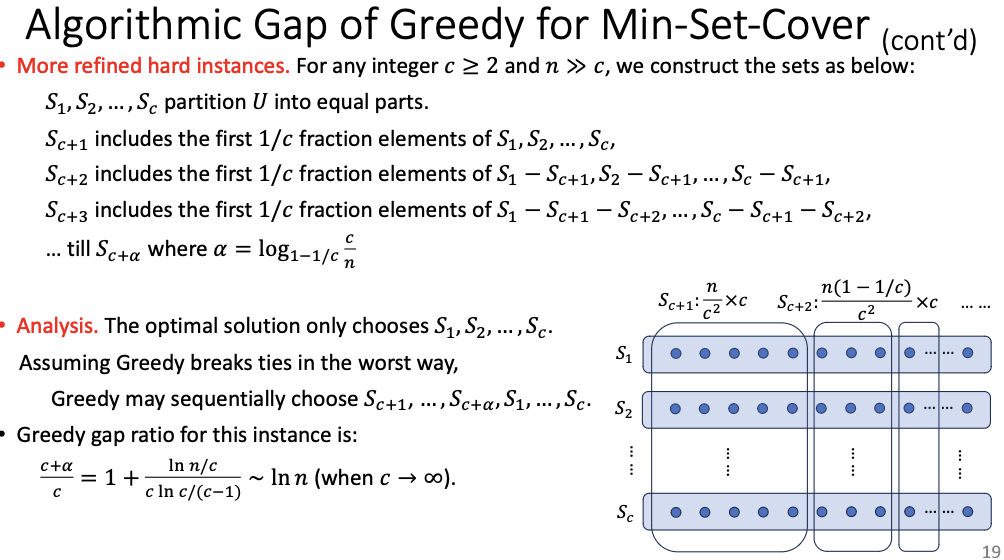
\includegraphics[width=\textwidth]{D11-set_cover_extreme_case.png}
    \caption{Extreme case for greedy algorithm}
\end{figure}
\subsection{Weighted Min Set-cover}
\begin{example}[Weighted Min Set-cover]
    Given  $ n $ elements,  $ M $ sets,  $ S_1,\cdots,S_M\subset U $. Each set  $ S_i $ has a weight  $ w(S_i)>0 $.

    Now select  $ T\subset\{S_1,\cdots, S_M\} $ such that  $ \dps\sum_{S\in T}w(S) $ minimized. 
\end{example}
Integer Program: Minimize  $ \dps\sum_{i=1}^M w(S_i)x_i $. Subject to   $ \dps\sum_{i:j\in S_i} x_i \geq 1$,  $ \forall j\in U $, where  $ x_i\in \{0,1\} $,  $ \forall i\in [M] $.

If we relax the integer constraint, we have an LP relaxation:  $ x_i\in[0,1] $, which can be solved in poly-time since it is a linear program.

We need "rounding" to transform fractional solution to the integer solution.

\subsubsection{Randomized Rounding}
If  $ \{x_i^*\} $ is the optimal LP solution.  For each  $ s_i $, select  $ s_i\in T $ independently with probability   $ \min\{\alpha x_i^*,1\} $. Then 
\[\Ebb[w(T)] \leq \alpha\sum_{i=1}^M w(s_i),\,x_i^*=\alpha\cdot \mathrm{LP} \leq \alpha\cdot \mathrm{OPT}\] 

Now we want to estimate  $ \mathrm{Pr}[T\text{ covers }U] $.

If there is some  $ \alpha x_i^ \geq 1 $, then  $ \mathrm{Pr}(T\text{ covers }U)=1 $. If  $ \forall i, x_i^*<1 $,   
then 
\[\begin{aligned}
    \mathrm{Pr}[T\text{ covers }U]&=1-\mathrm{Pr}[ \exists j\in U , j\not\in T ]\\
    & \geq 1-\sum_{j\in U}\mathrm{Pr}[j\not\in T]\\
    &=1-\sum_{j\in U}\prod_{i: j\in S_i}(1-\min\{\alpha x_i^*,1\})\\
    & \geq 1-\sum_{j\in U}\prod_{i: j\in S_i}\exp(-\alpha x_i^*)\qquad\text{(If some $ x_i^*<1 $, the probability will be 0)}\\
    &=1-\sum_{j\in U}\exp(-\sum_{j\in S_i}\alpha x_i^*)\\
    &=1-\sum_{j\in U}\exp(-\alpha)
\end{aligned}\]

Therefore, we obtain 
\begin{claim}
    \[\mathrm{Pr}(\text{every element covered}) \geq 1-n\cdot e^{-\alpha}\]
\end{claim}
If we set  $ \alpha=\ln n+\ln\ln n $, then 
\begin{align*}
    \mathrm{Pr}[\epsilon_1]\mathrm{Pr}[\text{every element covered}]&\geq 1-n\cdot e^{-\ln n-\ln\ln n}\\
    &=1-\frac{1}{n\ln n}\\
    &\geq 1-\frac{1}{\ln n}
\end{align*} 
We should also focus on  $ \Ebb(w(T)) \leq \alpha\cdot\OPT $. Here we use the \name{Markov Inquality}:
\begin{theorem}[Markov Inequality]
    For Random Variable  $ X \geq 0 $,  $ \mathrm{Pr}(X \geq t\mathbb EX) \leq \frac{1}{t} $  
\end{theorem} 
\begin{proof}
    \begin{align*}
        \Ebb X&=\Ebb[X|X \geq \alpha]\cdot \mathrm{Pr}(X \geq \alpha)+ \Ebb[X|X < \alpha]\cdot \mathrm{Pr}(X < \alpha)\\
        & \geq \alpha\cdot\mathrm{Pr}[X \geq \alpha]
    \end{align*}
    Therefore,  $ \mathrm{Pr}[X \geq \alpha] \leq \frac{\Ebb X}{\alpha} $ 
\end{proof}
So 
\begin{align*}
    \mathrm{Pr}[\epsilon_2]\mathrm{Pr}\left[\sum_{i}w(S_i)y_i\geq (\ln n+2\ln\ln n)\OPT\right]& \leq \frac{\ln n+\ln\ln n}{\ln n+2\ln \ln n} \\
    &=1-\frac{\ln \ln n}{\ln n+2\ln\ln n}
\end{align*}
So the union probablity 
\[\begin{aligned}
    \mathrm{Pr}[\epsilon\wedge \bar{\epsilon}_2]& \geq \mathrm{Pr}[\epsilon_1]-\mathrm{Pr}[\epsilon_2]\\
    & \geq \frac{\ln\ln n}{\ln n+2\ln\ln n}-\frac{1}{\ln n}\\
    & \geq \Omega(\frac{\ln\ln n}{\ln n})\xrightarrow{\text{boost}}1-\frac{1}{n^{100}}
\end{aligned}\]

\begin{theorem}
    With probability  $ \Omega(\frac{\ln\ln n}{\ln n}) $, LP+randomized rounding returns a  $ (\ln n+2\ln \ln n) $-approximation solution.  
\end{theorem}

The question is how to boost the probability. Indeed, if we independently round  $ N  $ times, 
\begin{align*}
    \mathrm{Pr}[\exists 1\text{ trial succeeds}]& \geq 1-[1-\Omega(\frac{\ln\ln n}{\ln n})]^N\\
    & \geq 1-\exp(-\Omega(\frac{\ln\ln n}{\ln n}\cdot N))\\
    & \geq 1-\exp(-\Omega(n\cdot\ln n)) \geq 1-e^{-n}
\end{align*}
if we set  $ N\leftarrow (\ln n)\cdot n $ in the last step.

Apply the method to Max-coverage problem, Integer Problem is to  $\max \dps\sum_{j=1}^n$ such that 
\begin{align*}
    \sum_{i=1}^M x_i &\leq k\\
    y_j& \leq \sum_{j\in S_i}x_i,\forall j\in [n]\\
    y_j& \leq 1,\forall j\in [n]\\
    x_i&\in\{0,1\},\forall i\in [M]
\end{align*} 
So the LP relaxation is to relax  $ x_i\in [0,1] $. 

Repeat  $ k  $ times and select set  $ i  $ with probability  $ \dps\frac{x_i^*}{k} $.

\begin{align*}
    \Ebb[\text{coverges}]& =\sum_{j=1}^n\mathrm{Pr}[j\text{ covered}]\\
    &=\sum_{j=1}^n\left(1-\left(1-\sum_{j\in S_i}\frac{x_i^*}{k}\right)^k\right)\\
    & \geq \sum_{j=1}^n\left(1-\exp(-\sum_{j\in S_i}x_i^*)\right)\\
    & \geq \sum_{j=1}^n\left(1-\exp(-y_i^*)\right)\\
    & \geq \alpha\sum_{j=1}^n y_j^*=\alpha\cdot \mathrm{LP} \geq \alpha\cdot \OPT
\end{align*}
where  $ \alpha=1-\frac{1}{e} $ 

The estimation is tight for this rounding if we consider the set  $ \mathcal{U}=\{0,1\}^k $ and  $ S_{i,0}=\{a\in U|a_i=0\} $,  $ S_{i,1}=\{a\in U|a_i=1\} $.   


\subsubsection{Integrality Gap}
Instance  $ I  $ is a  $ c $ vs.  $ s $-\name{Integrality Gap (IG) instance} if  $ \mathrm{LP}(I) \geq c $ and  $ \OPT(I) \leq s $. The \name{gap ratio} is  $\dps \frac{c}{s} $. 

\begin{enumerate}
    \item Large IG $ \Rightarrow  $ Inaccurate estimation of LP.
    \item The estimation of rounding algorithm is usually 
    \[\mathrm{rounding } \geq \cdots \geq \alpha\cdot\mathrm{LP} \geq \alpha\cdot\OPT\]
    Since  $ \mathrm{rounding} \leq \OPT $ in maximization problem, if IG is large,  $ \alpha $ can be very large and hence the approximation ratio is very bad. 
\end{enumerate}

For instance, consider the set-cover problem that is to minimize  $ \dps\sum_{i=1}^M x_i $ \st 
\[\sum_{j\in S_i}x_i \geq 1,\forall j\in U,\quad x_i\in [\{0,1\},\forall i\in [M]]\] 
relax the condition  $ x_i\in [0,1] $ and consider the set  $ \mathcal{U}=\{0,1\}^q\setminus\{0\} $ and  $ S_{\vec{\alpha}}=\{l\in U:l^T\alpha=1\pmod 2\} $ for  $ \alpha\in \{0,1\}^q $ with the size  $  M=2^q,n=2^q-1 $. 

\[|S_{\vec{\alpha}}|=\begin{cases}
    2^{q-1}&\alpha\neq 0\\
    0&\alpha=0
\end{cases}\]

\begin{claim}
    LP=2
\end{claim}
\begin{proof}
    Take  $ x_{\vec{\alpha}}=\frac{2}{2^q} $. Then  $ \dps\sum_{\vec{\alpha}}S_{\vec{\alpha}}=2 $. And the LP constraint met where
    \[\forall \vec{e}\in U,\,\sum_{\vec{e}\in S_{\vec{\alpha}}}\frac{2}{2^q}=2\mathrm{Pr}_{\vec{\alpha}\in \{0,1\}^q}[\vec{e}\in S_{\vec{\alpha}}]=2\times \frac{1}{2}=1\] 
    
    Certainly  $ \mathrm{LP} \geq 2 $, so  $ \mathrm{LP}=2 $.  
\end{proof}

But we also have a claim about  $ \OPT $:

\begin{claim}
     $ \OPT \geq q $. So the instance is a  $ 2 $ vs.  $ q $ IG with ratio  $ \frac{q}{2}=\frac{1}{2}\log_2(n+1)=\frac{\ln(n+1)}{2\ln 2} $.   
\end{claim}
\begin{proof}
    For any  $ S_{\vec{\alpha}_1},\cdots,S_{\vec{\alpha}_{q-1}} $, suppose  $ S_{\vec{\alpha}_1}\cup\cdots\cup S_{\vec{\alpha}_{q-1}} $ is a cover of  $ U $. Then 
    \begin{align*}
        &\Leftrightarrow \bar{S}_{\vec{\alpha}_1}\cap\cdots\cap\bar{S}_{\vec{\alpha}_{q-1}}=\{\vec{0}\}\\
        &\Leftrightarrow\{\vec{e}\in \{0,1\}^q:e^T\vec{\alpha}_i=0\forall i\in [q-1]\}=\{\vec{0}\}
    \end{align*} 
    which is impossible!
\end{proof}

%!TEX root = /lecture/Discrete_Optimistic.tex

Therefore, we obtain 
\begin{claim}
    \[\mathrm{Pr}(\text{every element covered}) \geq 1-n\cdot e^{-\alpha}\]
\end{claim}
If we set  $ \alpha=\ln n+\ln\ln n $, then 
\begin{align*}
    \mathrm{Pr}[\epsilon_1]\mathrm{Pr}[\text{every element covered}]&\geq 1-n\cdot e^{-\ln n-\ln\ln n}\\
    &=1-\frac{1}{n\ln n}\\
    &\geq 1-\frac{1}{\ln n}
\end{align*} 
We should also focus on  $ \Ebb(w(T)) \leq \alpha\cdot\OPT $. Here we use the \name{Markov Inquality}:
\begin{theorem}[Markov Inequality]
    For Random Variable  $ X \geq 0 $,  $ \mathrm{Pr}(X \geq t\mathbb EX) \leq \frac{1}{t} $  
\end{theorem} 
\begin{proof}
    \begin{align*}
        \Ebb X&=\Ebb[X|X \geq \alpha]\cdot \mathrm{Pr}(X \geq \alpha)+ \Ebb[X|X < \alpha]\cdot \mathrm{Pr}(X < \alpha)\\
        & \geq \alpha\cdot\mathrm{Pr}[X \geq \alpha]
    \end{align*}
    Therefore,  $ \mathrm{Pr}[X \geq \alpha] \leq \frac{\Ebb X}{\alpha} $ 
\end{proof}
So 
\begin{align*}
    \mathrm{Pr}[\epsilon_2]\mathrm{Pr}\left[\sum_{i}w(S_i)y_i\geq (\ln n+2\ln\ln n)\OPT\right]& \leq \frac{\ln n+\ln\ln n}{\ln n+2\ln \ln n} \\
    &=1-\frac{\ln \ln n}{\ln n+2\ln\ln n}
\end{align*}
So the union probablity 
\[\begin{aligned}
    \mathrm{Pr}[\epsilon\wedge \bar{\epsilon}_2]& \geq \mathrm{Pr}[\epsilon_1]-\mathrm{Pr}[\epsilon_2]\\
    & \geq \frac{\ln\ln n}{\ln n+2\ln\ln n}-\frac{1}{\ln n}\\
    & \geq \Omega(\frac{\ln\ln n}{\ln n})\xrightarrow{\text{boost}}1-\frac{1}{n^{100}}
\end{aligned}\]

\begin{theorem}
    With probability  $ \Omega(\frac{\ln\ln n}{\ln n}) $, LP+randomized rounding returns a  $ (\ln n+2\ln \ln n) $-approximation solution.  
\end{theorem}

The question is how to boost the probability. Indeed, if we independently round  $ N  $ times, 
\begin{align*}
    \mathrm{Pr}[\exists 1\text{ trial succeeds}]& \geq 1-[1-\Omega(\frac{\ln\ln n}{\ln n})]^N\\
    & \geq 1-\exp(-\Omega(\frac{\ln\ln n}{\ln n}\cdot N))\\
    & \geq 1-\exp(-\Omega(n\cdot\ln n)) \geq 1-e^{-n}
\end{align*}
if we set  $ N\leftarrow (\ln n)\cdot n $ in the last step.

Apply the method to Max-coverage problem, Integer Problem is to  $\max \dps\sum_{j=1}^n y_j$ such that 
\begin{align*}
    \sum_{i=1}^M x_i &\leq k\\
    y_j& \leq \sum_{j\in S_i}x_i,\forall j\in [n]\\
    y_j& \leq 1,\forall j\in [n]\\
    x_i&\in\{0,1\},\forall i\in [M]
\end{align*} 
So the LP relaxation is to relax  $ x_i\in [0,1] $. 

Repeat  $ k  $ times and select set  $ i  $ with probability  $ \dps\frac{x_i^*}{k} $.

\begin{align*}
    \Ebb[\text{coverges}]& =\sum_{j=1}^n\mathrm{Pr}[j\text{ covered}]\\
    &=\sum_{j=1}^n\left(1-\left(1-\sum_{j\in S_i}\frac{x_i^*}{k}\right)^k\right)\\
    & \geq \sum_{j=1}^n\left(1-\exp(-\sum_{j\in S_i}x_i^*)\right)\\
    & \geq \sum_{j=1}^n\left(1-\exp(-y_i^*)\right)\\
    & \geq \alpha\sum_{j=1}^n y_j^*=\alpha\cdot \mathrm{LP} \geq \alpha\cdot \OPT
\end{align*}
where  $ \alpha=1-\frac{1}{e} $ 

The estimation is tight for this rounding if we consider the set  $ \mathcal{U}=\{0,1\}^k $ and  $ S_{i,0}=\{a\in U|a_i=0\} $,  $ S_{i,1}=\{a\in U|a_i=1\} $.   


\subsubsection{Integrality Gap}
Instance  $ I  $ is a  $ c $ vs.  $ s $-\name{Integrality Gap (IG) instance} if  $ \mathrm{LP}(I) \geq c $ and  $ \OPT(I) \leq s $. The \name{gap ratio} is  $\dps \frac{c}{s} $. 

\begin{enumerate}
    \item Large IG $ \Rightarrow  $ Inaccurate estimation of LP.
    \item The estimation of rounding algorithm is usually 
    \[\mathrm{rounding } \geq \cdots \geq \alpha\cdot\mathrm{LP} \geq \alpha\cdot\OPT\]
    Since  $ \mathrm{rounding} \leq \OPT $ in maximization problem, if IG is large,  $ \alpha $ can be very large and hence the approximation ratio is very bad. 
\end{enumerate}

For instance, consider the set-cover problem that is to minimize  $ \dps\sum_{i=1}^M x_i $ \st 
\[\sum_{j\in S_i}x_i \geq 1,\forall j\in U,\quad x_i\in [\{0,1\},\forall i\in [M]]\] 
relax the condition  $ x_i\in [0,1] $ and consider the set  $ \mathcal{U}=\{0,1\}^q\setminus\{0\} $ and  $ S_{\vec{\alpha}}=\{l\in U:l^T\alpha=1\pmod 2\} $ for  $ \alpha\in \{0,1\}^q $ with the size  $  M=2^q,n=2^q-1 $. 

\[|S_{\vec{\alpha}}|=\begin{cases}
    2^{q-1}&\alpha\neq 0\\
    0&\alpha=0
\end{cases}\]

\begin{claim}
    LP=2
\end{claim}
\begin{proof}
    Take  $ x_{\vec{\alpha}}=\frac{2}{2^q} $. Then  $ \dps\sum_{\vec{\alpha}}S_{\vec{\alpha}}=2 $. And the LP constraint met where
    \[\forall \vec{e}\in U,\,\sum_{\vec{e}\in S_{\vec{\alpha}}}\frac{2}{2^q}=2\mathrm{Pr}_{\vec{\alpha}\in \{0,1\}^q}[\vec{e}\in S_{\vec{\alpha}}]=2\times \frac{1}{2}=1\] 
    
    Certainly  $ \mathrm{LP} \geq 2 $, so  $ \mathrm{LP}=2 $.  
\end{proof}

But we also have a claim about  $ \OPT $:

\begin{claim}
     $ \OPT \geq q $. So the instance is a  $ 2 $ vs.  $ q $ IG with ratio  $ \frac{q}{2}=\frac{1}{2}\log_2(n+1)=\frac{\ln(n+1)}{2\ln 2} $.   
\end{claim}
\begin{proof}
    For any  $ S_{\vec{\alpha}_1},\cdots,S_{\vec{\alpha}_{q-1}} $, suppose  $ S_{\vec{\alpha}_1}\cup\cdots\cup S_{\vec{\alpha}_{q-1}} $ is a cover of  $ U $. Then 
    \begin{align*}
        &\Leftrightarrow \bar{S}_{\vec{\alpha}_1}\cap\cdots\cap\bar{S}_{\vec{\alpha}_{q-1}}=\{\vec{0}\}\\
        &\Leftrightarrow\{\vec{e}\in \{0,1\}^q:e^T\vec{\alpha}_i=0\forall i\in [q-1]\}=\{\vec{0}\}
    \end{align*} 
    which is impossible!
\end{proof}

 $ I  $ is an  $ \alpha  $-Integrality Gap instance if 
 \[\mathrm{LP}(I) \leq \frac{1}{\alpha}\cdot\OPT(I)\]


Then we indeed prove that  $ \alpha $ can be  $\dps \frac{1}{2}\log_2(n+1)<\ln(n+1) $  in Min-Set-Cover problem.  



%!TEX root = /lecture/Discrete_Optimistic.tex

Take  $ U=\{1,2,\cdots,n\} $.  $ M  $ are  $ C\cdot  k\ln n $  sets, each of which  $ s_i $ includes each  $ j\in U $ independently with probability  $ \dps\frac{1}{k} $   

\begin{claim}
    When  $ C \geq \frac{4}{\epsilon^2} $, the probability 
    \[\mathrm{Pr}[\mathrm{LP}  \leq \frac{k}{1-\epsilon}]1-\frac{1}{n}\]
\end{claim}
\begin{proof}
    Consider  $ x_i=\dps\frac{k}{<(1-\epsilon)} $.
    
    Fix  $ j\in [n] $.
    \begin{align*}
        \mathrm{Pr}[\sum_{j\in S_i}x_i \geq 1]&=\mathrm{Pr}\left[\sum_{i=1}^M\mathbf{1}[j\in S_i] \geq \frac{(1-\epsilon)M}{k}\right]\\
        & \geq 1-\left[\frac{e^{-\epsilon}}{(1-\epsilon)^{1-\epsilon}}\right]^{\frac{M}{k}}\\
        &=1-\exp\left((-\epsilon-(1-\epsilon)\ln (1-\epsilon))\cdot\frac{M}{k}\right)\\
        & \geq 1-\exp(-\frac{\epsilon^2}{2}\cdot\frac{M}{k})\\
        & \geq 1-\exp(-2\ln n)
    \end{align*} 
    Here we use the Chernoff bound with a high relation of central limit theorem.
    \begin{theorem}[Chernoff Bound]
        $ X_1,X_2,\cdots,X_n\in [0,1] $ a.s. and  $ \Ebb X_i=p_i $. Let  $ X=X_1+\cdots+X_n $,  $ \Ebb X=\mu $. For any  $ \delta>0 $
        \[\begin{cases}
            \mathrm{Pr}[X \geq (1+\delta)\mu] \leq \left[\frac{e^\delta}{(1+\delta)^{1+\delta}}\right]^\mu\\
            \mathrm{Pr}[X \leq (1-\delta)\mu] \leq \left[\frac{e^{-\delta}}{(1-\delta)^{1-\delta}}\right]^\mu
        \end{cases}\]    
    \end{theorem}
\end{proof}

\begin{claim}
    For  $ k \geq \frac{2}{\epsilon} $ and  $ n=n(k,\epsilon,C) $ large enough, we have 
    \[\mathrm{Pr}[\OPT \geq (1-\epsilon)k\ln n] \geq 0.99\]  
\end{claim}

\begin{proof}
    Let  $ z=(1-\epsilon)k\ln n $.
    
    $ \OPT>z $ $ \Leftarrow $  $ \forall \mathcal{S}\in\binom{[M]}{z} $,  $ \mathcal{S}  $ doesn't cover  $ U $. We consider probability of the latter case.

    Now fix  $ \mathcal{S}\in \binom{[M ]}{z} $,  $ \mathrm{Pr}[\mathcal{S}\text{ cover }U] $ is actually 
    \begin{align*}
        \mathrm{Pr}[\mathcal{S}\text{ cover }U]&=\mathrm{Pr}[\forall j\in U,\exists S_i\in \mathcal{S},j\in S_i]\\
        &=\mathrm{Pr}[\exists S_i\in \mathcal{S},1\in S_i]^n\\
        &=\left(1-(1-\frac{1}{k})^z\right)^n\\
        & \leq \exp(-n(1-\frac{1}{k})^z)\\
        & \overset{k \geq 2}{ \leq } \exp(-n\exp(-(1-\epsilon)(1+\frac{1}{k})\ln n))\\
        & \overset{k \geq \frac{2}{\epsilon }}{ \leq } \exp(-n\exp(-(1-\frac{\epsilon}{2})\ln n))\\
        &=\exp(-n\cdot n^{-(1-\frac{\epsilon}{2})})\\
        &=\exp(-n^{\frac{\epsilon}{2}})
    \end{align*}
    So 
    \begin{align*}
        \mathrm{Pr}[\exists \mathcal{S}\in\binom{[M]}{z},\mathcal{S}\text{ cover }U]& \leq \binom{M}{z}\cdot\exp(-n^{\frac{\epsilon}{2}})\\
        & \leq \left(\frac{C\cdot e}{1-\epsilon}\right)^{(1-\epsilon)k\ln n}\cdot \exp(-n^{\frac{\epsilon}{2}})\\
        &<\exp(-n^{\frac{\epsilon}{4}})\\
        &<0.01
    \end{align*}
    as  $ n  $ large enough.
    Here we end the proof
\end{proof}


So using Randomized construction,  $ \alpha $ can approach  $ (1-\epsilon)\ln n $ for any  $ \epsilon $.

\subsection{Hardness of  Approximation}
\subsubsection{ P,NP classes}
For  $ \mathcal{L }\in \{0,1\}^\ast       $ is  the  $ 0-1 $ encoding, a problem is the set of some  $ 0-1 $ encoding and a decision problem is to decide whether  $ \mathcal{L} $ belongs to it. 

For instance, $ \mathcal{L}_k $  is the set of all ($ 0-1 $ encoding) of set cover instances where  $ U  $ can be covered by  $ k  $ sets. We define 
\begin{center}
    $ \dps P=\{\mathcal{L}:\mathcal{L}\text{ can be poly-time decided by a (deterministic) Turing machine}\} $ 
\end{center}
\begin{center}
    $ \dps NP=\{\mathcal{L}:\mathcal{L}\text{ can be poly-time decided by a non-deterministic Turing machine}\} $
\end{center}

NP problems are all problems that can be "verified" in poly-time. Explicitly,

for input instance  $ x\in \{0,1\}^\ast $, the prover is based on  $ x $, providing a "proof"  $ y\in \{0,1\}^\ast $ that  $ |y| \leq \mathrm{poly}(|x|) $, however, the verifier is a poly-time algorithm that accepts   $ x,y  $ and outputs YES/NO.

In other words,  $ \mathcal{L}\in  $ NP  $ \Leftrightarrow $   $ \exists $ a prover-verifier system such that 
\begin{itemize}
    \item Completeness:  $ \forall x\in \mathcal{L} $,  $ \exists $ proof $ y $ \st verifier returns YES in poly-time.
    \item Soundness: $ \forall x\not\in \mathcal{L} $, $ \forall  $  proof  $ y $, verifier returns  NO in poly-time.     
\end{itemize} 
The equivalence is because we actually can "guess" the proof  $ y  $ in a non-deterministic TM.

If P=NP, then if we can verify  proof in poly-time, we can also construct it in poly-time. There isn't innovation anymore!

\name{NP-complete}:  $ \mathcal{L} $ is NPC if 
\begin{enumerate}[label=\arabic*)]
    \item  $ \mathcal{L}\in  $ NP 
    \item  $ \forall  $  $ \mathcal{L}'\in  $ NP,  $ \mathcal{L}' \geq_p\mathcal{L} $ \ie  $ \mathcal{L}' $ can be reduced to  $ \mathcal{L} $ in poly-time.      
\end{enumerate} 

Equivalently, if some NPC problems can be solved in poly-time, then P=NP.

If only 2) in the definition of NPC holds, then it is a \name{NP-hard} problem.

%!TEX root = /lecture/Discrete_Optimistic.tex

We define the \name{polynomial reduction}  $ M \leq _p L $ if 

$ \exists  $ poly-time algorithm  $ A $ such that  $ \forall x\in \{0,1\}^* $,
\begin{itemize}
    \item (completeness)  $ x\in M $ returns YES $ \Rightarrow A(x)\in L $ returns YES.
\item (soundness)  $ x\in M $ returns NO $ \Rightarrow  $  $ A(x)\in L $  returns NO.  
\end{itemize} 

Observed that if  $ M  $ is NP-Complete and  $ M \leq_p\mathcal L  $, then  $ L $ is NP-Hard.


\begin{theorem}[Cock-Levin]
    3-SAT is NP-Complete.
\end{theorem}
\begin{proof}
    $ \forall L\in NP $, need to show  $ L \leq_p  $ 3-SAT.
    
    Let  $ A  $ be the poly-time verifier (DTM) for  $ L $.

    Now we consider the original DFA, which needs start, process and after, denoted as  $ (s,p,\alpha) $ 

    For time  $ t $, the tape can be 
    \[t_{-M}^{(t)},\cdots,t_M^{(t)},\alpha^{(t)},S^{(t)},p^{(t)}\]

    where the transition function is 
    \begin{align*}
        t_i^{(\tau)}&=g_i(t_i^{(\tau-1)},\alpha^{(\tau-1)},s^{(\tau-1)},p^{(\tau-1)})\\
        s^{(\tau)}&=h_(\alpha^{(\tau-1)},s^{(\tau-1)},p^{(\tau-1)})\\
        p^{(\tau)}&=\cdots\\
        \alpha^{(\tau)}&=\cdots
    \end{align*}

    which is a compose of bool function. So any DFA process can be converted to a 3-SAT instance.
    
\end{proof}

\begin{theorem}[Max-Coverage]
    Deciding whether Max-Coverage=100\% is NP-Complete.
\end{theorem}
\begin{proof}
    We divide it into two parts:
    \begin{enumerate}[label=\arabic*.]
        \item Max-coverage=1 is NP.
        \item 3-SAT  $  \leq _p $ Max-coverage=1. 
    \end{enumerate}
    Consider any  $ 3 $-SAT instance  $ I $. We have variables  $ x_1,\cdots,x_n $ and clauses  $ c_1,\cdots,c_m $.  

    Denote  $ U=\{x_1,\cdots,x_n,c_1,\cdots,c_m\} $ and sets $ S_1,S_2,\cdots,S_n,S_{n+1},\cdots,S_{2n} $. For  $ i=1,2,\cdots,n $, 
    \[S_i=\{x_i\}\cup\{c_j:c_j\text{ contains }x_i\}\]
    \[S_{n+i}=\{x_i\}\cup\{c_j:c_j\text{contains}\bar{x}_i\}\]
    Let  $ k=n $.   

    Completeness: If  $ I $ satisfiable, then $ \exists \sigma:\{x_i\}\rightarrow \{0,1\} $, choose  $ \begin{cases}
        S_i&\text{if  $ \sigma(x_i)=1 $ }\\
        S_{n+i}&\text{if  $ \sigma(x_i)=0 $ }\\
    \end{cases} $   
    
    Soundness: If  $ J $ is YES, for  $ I $, let  $ \sigma(x_i)=\begin{cases}
        1&\text{if  $ S_i $ chosen}\\
        0&\text{if  $ S_{i+n} $ chosen}\\
    \end{cases} $.
\end{proof}

Now we want to consider the approximation problem.

1 vs. 1 Max-Coverage is NP-H but what if decide  the gap-version  $ s $ vs.  $ c $.

\paragraph{Observation} If we could prove  $ c $ vs.  $ s $ M-C is NP-H for  $ c >s $. Then  $ \frac{s}{c} $ approximation M-C problem is NP-H.  

\begin{theorem}[PCP theorem]
    $ \exists \epsilon $ \st  $ \mathrm{Max-3-SAT}_{1,1-\epsilon} $ is NP-Hard.
\end{theorem}

We give an introduction for PCPs.

\begin{definition}[Probability Checkable Proofs]
    Verifier: input instance  $ x $ and proof  $ y $.
    
    Reads  $ x $, compute a (joint) distribution $ D $  over the locations in  $ y $, and a Boolean function.
    
    Sample  $ i,j,k,f \sim D $.

    output YES iff  $ f(y_i,y_j,y_k)=1 $.

    \begin{itemize}
        \item (completeness) If  $ x  $ is YES, then  $ \exists  $  $ y $ \st  $ \mathrm{Pr}[\text{Verifier accepts}] \geq c $.
        \item (soundness) If  $ x $ is NO, then  $ \forall y $, 4
        $ \mathrm{Pr}[\text{Verifier accepts}]  \leq s$.    
    \end{itemize}
\end{definition}

Then PCP theorem is equivalent to 
\begin{theorem}[PCP theorem]
    $ \exists \epsilon>0 $ \st every NP problem has a PCP system with  $ c=1 $,  $ s=1-\epsilon $.   
\end{theorem}

\begin{definition}
    $ \mathrm{PCP}_{c,s}[r,q] $ denotes set of languarges that admits a PCP system with  $ c,s,r,q  $ parameters. Explicitly,
    \begin{itemize}
        \item Prover reads input, outputs poly-length proof with unbounded computational prover.
        \item Verifier in poly-time reads input and  $ r $ random bits, (deterministically by input and random bits) computes  $ q $ locations in the proof, reads the  $ q $ bits in the proof and decides YES/NO.
        \item The systems satisfies  completeness and soundness:
        \begin{itemize}
            \item (Completeness) Input is YES instance  $ \Rightarrow  $  $ \exists\,\text{ prover}\mathrm{Pr}[\text{Verifier accepts}] \geq c $.
            \item (Soundness) Input is NO instance  $ \Rightarrow  $  $ \forall\,\text{ prover}\mathrm{Pr}[\text{Verifier accepts}] \leq s $. 
        \end{itemize}
    \end{itemize}
\end{definition}
\begin{observation}
    \,
    \begin{itemize}
        \item  $ \mathrm{PCP}_{1,\frac{1}{2}}[0,0]=P $.
        \item  $ \mathrm{PCP}_{1,\frac{1}{2}}[0,\mathrm{poly(n)}]=NP $.
        \item  $ \mathrm{PCP}_{1,\frac{1}{2}}[O(\log(n)),O(1)] \leq NP $   
    \end{itemize}
\end{observation}
For the final observation, we actually can construct a Verifier to enumerate all possible random bits in $ \{0,1\}^r $ to return YES if there is some possibility larger than  $ c $.

Indeed, PCP theorem is actually,
\begin{theorem}[PCP theorem]
    \[\mathrm{PCP}_{1,\epsilon}[O(\log n),O(1)]=\mathrm{PCP}_{1,\frac{1}{2}}[O(\log n),O(1)]=NP \]
\end{theorem}

\begin{proposition}
    PCP theorem  $ \Leftrightarrow $   $ \exists s<1,\mathrm{Gap-3MAXSAT}_{1,s} $ is NP-Hard.
\end{proposition}
\begin{proof}
    " $ \Rightarrow $ ": Our goal is to prove  $ \mathrm{3SAT} \leq_p \mathrm{Gap-3MAXSAT}_{1,s} $,\ie given a 3-SAT instance  $ \phi $, we can construct an instance $ \Phi $ in poly-time  such that  $ \mathrm{OPT}(\phi)=1 $ $ \Rightarrow  $  $ \OPT(\Phi)=1 $.
    
    $ \mathrm{3SAT}=\mathrm{GAP-3MAXSAT}_{1,\frac{1}{m}}$ is NP-hard. By PCP theorem,  $ \exists  $ a prover-verifier system for 3-SAT that with  $ c=1,s=\frac{1}{2},r=O(\log n),q=O(1) $ 
    
    Prover provides proof  $ \vec{x}\in \{0,1\}^N $.

    Given  $ \phi $,  $ \forall \vec{\tau}\in \{0,1\}^r $, verifier computes 
    \[l_1,\cdots,l_q\in \{1,2,\cdots,N\}\]
    \[f:\{0,1\}^q\rightarrow \{0,1\}\]
    find  $ 3-CNF $  $ g $ over  $ q+q\cdot 2^q $ variables $ \{z_{\vec{\tau}}\} $  and  $ q\cdot 2^q $ clauses $ c_{\vec{\tau}} $  such that  $ f(\vec{y})=1 $ iff  $ \exists \vec{z}\in \{0,1\}^{q\cdot 2^q},g(\vec{y},\vec{z})=1 $.       
    
    Construct  $ \Phi $ with variables  $ \{x_1,x_2,\cdots,x_N\}\cup \bigcup_\tau z_{\tau} $ and clauses  $\bigwedge_\tau c_{\tau} $.

    Completeness: If  $ \exists \vec{x} $  such that  $ \mathrm{Pr}_{\vec{\tau}}[\text{Verifier accepts}]=1 $. Then  $ \forall \vec{\tau}$,  $ \exists z_{\vec{\tau}} $ such that  $ c_{\vec{\tau}}=1 $.    

    Soundness:  $ \forall \vec{x},\mathrm{Pr}_{\vec{\tau}}[\text{Verifier accepts}] \leq \frac{1}{2} $. Consider a solution $ \sigma $  to  $ \Phi $.  Let  $ T=\{\vec{\tau}:\text{ Verifier rejects  $ \sigma(X) $ under  $ \vec{\tau} $}\} $. Then  $ T \geq \frac{1}{2}\cdot 2^r $.
    
    $ \forall \vec{\tau} $,  $ \sigma  $ doesn't satisfy all clauses in  $ C_{\vec{\tau}} $ so the number of unsatisfied clauses  $  \geq |T|=\frac{1}{2}\cdot 2^r $.
    
    \[\val(\sigma:\Phi) \leq 1-\frac{|T|}{2^r\cdot q\cdot 2^q}=1-\frac{\frac{1}{2}\cdot 2^r}{2^r\cdot q\cdot 2^q}=1-\frac{1}{2q\cdot 2^q}\]

    " $ \Leftarrow $ ":  $ \forall  $ NP language  $ \mathcal{L} \leq_p \mathrm{GAP-3SAT}_{1,s}$. Then 
    \[\mathcal{L}\in \mathrm{PCP}_{1,s}[O(\log n),3] \leq \mathrm{PCP}_{1,\frac{1}{2}}[O(\log (n),O(1))]\] 
\end{proof}

\begin{theorem}\label{thm:gap3sat}
    $ \forall \epsilon>0 $,  $ \mathrm{GAP-3SAT}_{1,\frac{7}{8}+\epsilon} $ is NP-Hard.  
\end{theorem}
\begin{corollary}
    $ \forall \epsilon>0 $,  $ (\frac{7}{8}+\epsilon) $-approximation Max3SAT is NP-Hard. 
\end{corollary}

The corollary is equivalent to  $ \forall \epsilon>0,\mathrm{Gap3SAT}_{1-\epsilon,\frac{7}{8}+\epsilon} $ is NP-Hard.

\begin{remark}
    It implies that  it is hard to find an algorithm better than random algorithm. It also shows that perfect completeness is sometimes very hard.
\end{remark}

\subsection{Label-Cover Games}

To prove the theorem, we need to consider a constraint Graph  $ G=(U,V,E) $, which is a bipartite graph. 

\underline{Prover} is a function  $ \sigma:U\rightarrow [K],V\rightarrow [L] $. 

\underline{Constraints}: For each  $ e=(u,v)\in E $,  $ \pi_e:[L]\rightarrow [K] $.

\underline{Verifier}: Uniformaly sample  $ e=(u,v)\in  E $, accepts only if  $ \pi_e(\sigma(v))=\sigma(u) $.

The system is also called  "2-Prover-1Verifier  Game" or "Projection Game".

More generally,  $ \pi_e\subset [K]\times [L] $.

\begin{claim}
    PCP Theorem implies that  $ \exists \delta>0 $,  $ \mathrm{Gap-LC}_{1,1-\delta}^{(K,L)=(2,7)} $ is NP-Hard.  
\end{claim}
\begin{proof}
    Reduce from  $ \mathrm{Gap-3SAT}_{1,1-\epsilon} $. 

        \begin{center}
        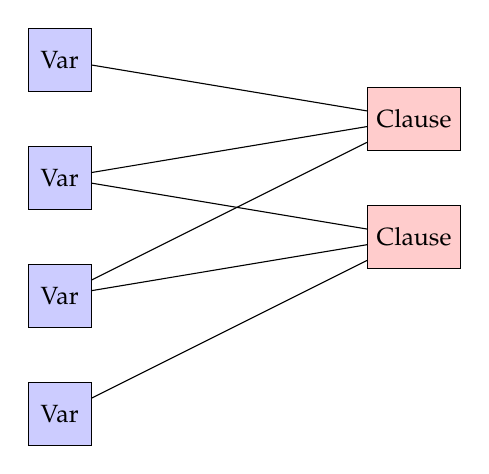
\begin{tikzpicture}[scale=1.5, every node/.style={draw, minimum size=0.8cm, font=\small}]
            % Variables (U)
            \node[fill=blue!20] (x1) at (0, 2) {Var};
            \node[fill=blue!20] (x2) at (0, 1) {Var};
            \node[fill=blue!20] (x3) at (0, 0) {Var};
            \node[fill=blue!20] (x4) at (0, -1) {Var};

            % Clauses (V)
            \node[fill=red!20] (c1) at (3, 1.5) {Clause};
            \node[fill=red!20] (c2) at (3, 0.5) {Clause};

            % Edges
            \draw[-] (x1) -- (c1);
            \draw[-] (x2) -- (c1);
            \draw[-] (x3) -- (c1);
            \draw[-] (x2) -- (c2);
            \draw[-] (x3) -- (c2);
            \draw[-] (x4) -- (c2);
        \end{tikzpicture}
        \end{center}

        Variables  $ x_i $ have  $ \sigma(x_i)\in \{0,1\} $ and Clauses  $ c_i=x_{j_i}^1\wedge x_{j_i}^2\wedge x_{j_i}^3 $ have  $ \sigma(c_i)\in [7] $ to represent the state of  $ c_i $.
    \end{proof}

\subsubsection{Paralled Repetition}
Given  $ H=\left(G(U,V,E),K,L,\{\pi_e\}\right) $.
\[H^{\otimes t}=\left(G^{\otimes t},K^t,L^t,\{\pi_{e_1,e_2,\cdots,e_t}\}\right)\]
where 
\[G^{\otimes t}=\{(u_1,u_2,\cdots,u_t),(v_1,v_2,\cdots,v_T)\}\] 

\[\pi_{(u_1,v_1),\cdots,(u_t,v_t)}=\left\{\left((\alpha_1,\cdots,\alpha_t),(\beta_1,\cdots,\beta_t)\right):(\alpha_i,\beta_i)\in \pi_{(u_i,v_i)}\right\}\]

It is easy to check that if  $ H  $ is a projection game,  $ H^{\otimes t} $ is also a projection game.

We wonder whether the following theorem holds
\begin{theorem}[not quite true]
    \[\OPT(H^{\otimes t}) \leq \OPT(H)^t\]
\end{theorem}
There is a counter-example for  $ U=\{u_1,u_2\},V=\{v_1,v_2\},K=L=4 $ and  $ G $ is fully connected. 
$ [K],[L]\leftrightarrow \{u,v\}\times\{1,2\} $ 

$ \pi_{(u_i,v_j)}=\{((u,i),(u,i)),((v,j),(v,j))\} $ 

Clearly,  $ \OPT(H)=\frac{1}{2} $.

However,  $ \OPT(H^{\otimes 2})=\frac{1}{2} $.

Let  $ \sigma((u_{i_1},u_{i_2}))=(((u,i_1),(v,i_1))) $,  $ \sigma((v_{j_2},v_{j_2}))=((u,j_1),(v,j_2)) $.  

So verifier accepts if  $ i_1=j_2 $.

However, the following theorem holds:
\begin{theorem}
    Suppose  $ H  $ has alphabet size less than  $ k $ and  $ \OPT(H) \leq 1-\delta $.  Then 
    \[\OPT(H^{\otimes t}) \leq \exp(-\Omega(\frac{\delta^3t}{\log K}))\]  
\end{theorem}
\begin{corollary}
     $ \forall \delta>0 $,  $ \exists  $   $ K,L $ such that  $ \mathrm{GAP-LC}(K,L)_{1,\delta} $ is NP-Hard.  
\end{corollary}

\begin{proof}[Proof of Theorem \ref{thm:gap3sat}]
    
\end{proof}

%!TEX root = /lecture/Discrete_Optimistic.tex

    Recall max-coverage problem is:  $ U=\{1,2,\cdots,n\} $,  $ S_1,S_2,\cdots,S_m\subset U,k \leq m $. Our goal is to select  $ k  $ sets to maximize  $ \dps\frac{1}{|U|}|\text{unon of selected sets}| $.
    
    We have proved that  $ (1-\frac{1}{e}) $-approximation is NP-hard.
    
\begin{theorem}
    $ \forall \epsilon>0 $,  $ \mathrm{Gap-MC}_{1,\frac{3}{4}+\epsilon} $ is NP-Hard.
\end{theorem}
\begin{proof}
    Suffices to reduce  $ LC $ case to  $ MC $ case.
    
    Let  $ W=\bigcup_{(u,v)\in E}T_{uv}\times\{(u,v)\} $,  $ |W|=2^k\cdot|E| $, where  $ T_{uv}=\{0,1\}^k $.
    
    Denotes 
    \[T_{uv,\alpha,0}=\{\vec{x}:x_\alpha=0\}\]
    \[T_{uv,\pi_{uv}(\beta),1}=\{\vec{x}:x_{\pi_{uv}(\beta)}=1\}\]


    Let  \[S_{u,\alpha}=\bigcup_{(u,v)\in E} T_{uv,\alpha,0}\times\{(u,v)\},\forall u\in U,\alpha\in [K] \]
    \[S_{v,\beta}=\bigcup_{(u,v)\in E}T_{uv,\pi_{uv}(\beta),1}\times\{(u,v)\},\forall v\in V,\beta\in [L]\]
    Take  $ k=|U|+|V| $.

    Completeness: $ \exists\sigma $ satisfies all constraints in  $ \mathrm{LC} $. Then select  $ \{S_{u,\sigma(u)},S_{v,\sigma(v)}\} $ to achieve 100\% coverage.
    
    Soundness: If  $ \OPT(LC)<\delta $,  $ \Rightarrow $  $ \OPT(MC)<\frac{3}{4}+\epsilon $.
    
    Otherwise, if  $ \exists $ set selection achieving  $ \frac{3}{4}+\epsilon $ coverage, then one can "decode" a  $ \sigma  $ such that   $ \mathrm{Val}(\sigma;\mathrm{LC}) \geq \delta $.

    Let 
    \[\mathrm{Sugg}(u)=\{\alpha,S_{u,\alpha}\text{ selected}\},\mathrm{Sugg}(v)=\{\beta:S_{v,\beta}\text{ selected}\}\]

    \begin{claim}
        \[\mathbb{E}_{(u,v)\sim E}\left[|\mathrm{Sugg}(u)|+|\mathrm{Sugg}(v)|\right]=2\]
    \end{claim}
    \begin{proof}[Proof of Claim]
        \begin{align*}
            \mathbb{E}_{(u,v)\sim E}\left[|\mathrm{Sugg}(u)|+|\mathrm{Sugg}(v)|\right] &= \sum_{(u,v)\in E}\frac{1}{|E|}\left(|\mathrm{Sugg}(u)|+|\mathrm{Sugg}(v)|\right)\\
            &= \Ebb_{u\sim U}|\mathrm{Sugg}(u)|+\Ebb_{v\sim V}|\mathrm{Sugg}(v)|\\
            &=\frac{1}{|U|}\left(\sum_u|\mathrm{Sugg}(u)|+\sum_v|\mathrm{Sugg}(v)|\right)\\
            &=2
        \end{align*}
    \end{proof}
    Here we use Corollary \ref{LC large theorem} with the stronger version that the graph is regular.

    \underline{Decoding Scheme}:  $ \forall u\in U $, choose  $ \sigma(u) $ uniformly from  $ \mathrm{Sugg}(u) $,  $ \forall v\in V $, choose  $ \sigma(v) $ uniformly from  $ \mathrm{Sugg(v)} $.

    \begin{definition}
        Edge  $ (u,v)\in E $ is \textit{consistently suggested} if  $ \exists \alpha\in \mathrm{Sugg}(u),\beta\in \mathrm{sugg}(v) $ such that  $ \pi_{uv}(\beta)=\alpha $.
        
        \begin{fact}
            If  $ (u,v)  $ is consistently suggested, then 
            \[\mathrm{Pr}_\sigma[(u,v)\text{ satisfied}] \geq \frac{1}{|\mathrm{Sugg}(u)|\cdot|\mathrm{Sugg}(v)|}\]
        \end{fact}
    \end{definition}
    Now consider 
    \[E_1=\{(u,v)\in E|(u,v)\text{ consisntently suggested}\}\]
    \[E_0=E\setminus E_1,\qquad \gamma=\frac{|E_1|}{|E|}\]
    \begin{lemma}
        If  $ (u,v)\in E_0 $, then 
        \[\text{coverage of }T_{uv} \leq 1-2^{-\left(|\mathrm{Sugg}(u)|+|\mathrm{Sugg}(v)|\right)}\]
    \end{lemma}
    \begin{proof}
        Note that if  $ |\mathrm{Sugg}(u)|=|\mathrm{Sugg}(v)|=1 $, then coverage of  $ T_{uv} \leq \frac{3}{4} $,
        
        \begin{align*}
            &\quad\,\text{non-coverage of  $ T_{u,v} $ }\\
            &=\mathrm{Pr}_{\vec{x}\sim\{0,1\}^k}\left[\forall \alpha\in \mathrm{Sugg}(u):x_\alpha=1\vee \forall \beta\in \mathrm{Sugg}(v):x_{\pi(\beta)}=0\right]\\
            &=\mathrm{Pr}_{\vec{x}\sim\{0,1\}^k}\left[\forall \alpha\in \mathrm{Sugg}(u):x_\alpha=1\right]\cdot\mathrm{Pr}_{\vec{x}\sim\{0,1\}^k}\left[\forall \beta\in \mathrm{Sugg}(v):x_{\pi(\beta)}=0\right]\\
            &=2^{-|\mathrm{Sugg}(u)|}\cdot2^{-|\pi(\mathrm{Sugg}(v))|}\\
            &   \geq 2^{-\left(|\mathrm{Sugg}(u)|+|\mathrm{Sugg}(v)|\right)}
        \end{align*}
    \end{proof}

    \begin{definition}
        Edge  $ (u,v) $ is  \textit{$ \tau $-good} if  $ \min\{|\mathrm{Sugg}(u)|,|\mathrm{Sugg}(v)|\} \leq \tau $. Then if  $ (u,v)\in E_1 $ and  $ \tau $-good, then  $ \mathrm{Pr}_\sigma[(u,v)\text{ satisfied by }\sigma] \geq \frac{1}{\tau^2} $     
    \end{definition}
    Let 
    \[\Ebb_{(u,v)\sim E_1}\left[|\mathrm{Sugg}(u)|+|\mathrm{Sugg}(v)|\right]=\tau\]

    Then at least  $ \frac{1}{2} $ edges in  $ E_1 $ are  $ (2\tau ) $-good.
    
    Then 
    \[\begin{aligned}
        \mathbb{E}_\sigma\left[\mathrm{Val}(\sigma;LC)\right]& \geq \gamma\cdot\frac{1}{2}\cdot\frac{1}{(2\tau)^2}
    \end{aligned}\]
    For the original Max-coverage problem, it subjects to 
    \[\begin{aligned}
        \frac{3}{4}+\epsilon& \leq \gamma\cdot 1+(1-\gamma)\left[1-\Ebb_{(u,v)\sim E_0}2^{-|\mathrm{Sugg}(u,v)|}\right]\\
        & \leq \gamma+(1-\gamma)\left[1-2^{-\Ebb_{(u,v)\sim E_0}|\mathrm{Sugg}(u,v)|}\right]\\
        &=\gamma+(1-\gamma)\left[1-2^{-\frac{2-\gamma\tau}{1-\gamma}}\right]
    \end{aligned}\]
    Suffices to prove a claim that 
    \begin{claim}
        If  $ \gamma+(1-\gamma)\left[1-2^{-\frac{2-\gamma\tau}{1-\gamma}}\right] \geq \frac{3}{4}+\epsilon $, then 
        \[\gamma \geq \frac{4}{1+\ln 4}\epsilon>\epsilon\]
        and 
        \[\tau \leq \frac{2}{\epsilon}\]
        So 
        \[\gamma\cdot\frac{1}{8\tau^2} \geq \epsilon\cdot\frac{\epsilon^2}{32}=\frac{\epsilon^3}{32}>\delta\]
    \end{claim}
    Here we prove that 
    \[\mathrm{Gap-MC}_{1,\frac{3}{4}+\epsilon}\xleftarrow{\delta=\epsilon^3/32}\mathrm{Gap-LC}(K,L)_{1,\delta}\]
\end{proof}

\subsection{Multicut}
\begin{example}[Multicut]
    Input: undirected graph  $ G=(V,E) $, weights  $ \omega:E\rightarrow\Rbb_{ \geq 0} $ and terminal pairs  $ \{(s_i,t_i)\}_{i=1}^k $.
    
    Our goal is to find  $ E'\subset E $ to  minimize  $ \omega(E')=\sum_{e\in E'}\omega(e) $ such that  $ s_i,t_i $ disconnected in  $ (V,E-E') $,  $ \forall i\in [k] $.     
\end{example}

Clearly,  $ k=1 $ is the min-cut problem.

\begin{theorem}
    $ k=2 $ can be solved in polynomial time. 
\end{theorem}
\begin{fact}
    $ k \geq 3 $, then  $ k $-approximation problem is easy. Actually, we can consider the union of all  min $ (s_i,t_i) $-cut.  
\end{fact}

\begin{example}[Vertex Cover]
    Input  $ G=(V,E) $.

    Our goal is to select  $ V'\subset V  $ to minimize  $ |V'| $ such that  $ \forall e\in E $,  $ e  $ has  $  \geq 1 $ endpoints in  $ V $.    
\end{example}

Those two problems are equivalent. Acutally,  $ \OPT(I)=\OPT(J) $ for two corresponding instances.


\begin{theorem}
    1.414-approximation for VC is NPH. Assuming UG-Conjecture,  $ (2-\epsilon) $-approximation is hard.

    As a result, 1.414-approximation for multicut is NPH. Assuming UGC, no poly-time constant approximation for multi-cut.
\end{theorem}

The goal in this lecture is to give a  $ O(\log n) $-approximation approximation. 

\subsubsection{Multicut on Trees}
Consider LP relaxation:
\[\min \sum_{e\in E }\omega(e)\cdot\chi_e\]
\[\st \sum_{e\in P(s_i,t_i)}\chi_e \geq 1\]
\[\chi_e \geq 0,\forall e\in E\]
where  $ P(s_i,t_i) $  is the unique path on tree.

\paragraph{Rounding} Let  $ d(v)=\dps\sum_{e\in P(r,v)}\chi_e,\forall v\in V $.

Sample  $ \theta\in [0,\frac{1}{2}) $ uniformly.

Say  $ \theta $ cuts  $ e=(u,v)  $ if  $ [d(u),d(v))\cap\{\theta,\theta+\frac{1}{2},\theta+1,\theta+\frac{3}{2},\cdots\}\neq \emptyset $.

Let   $ E'=\{e\in E\text{ cut by  $ \theta $}\} $.

\underline{Feasiblity}: Consider any  $ (s_i,t_i) $. Let  $ u_i $ be the least common ancestor of  $ s_i,t_i $.  Then 
\[d(s_i)-d(u_i)+d(t_i)-d(u_i) \geq 1\]
Assume WLOG  $ d(s_i)-d(u_i) \geq \frac{1}{2} $. Then  $ P(s_i,u_i)\cap E'\neq \emptyset $.

\underline{Quality}: Consider  $ e=(u,v) $,
\[\mathrm{Pr}[e\text{ cut by }\theta]=\begin{cases}
    1&\chi_e \geq \frac{1}{2}\\
    2\chi_e&\chi_e<\frac{1}{2}
\end{cases}\]

\[\Ebb_\theta \omega(E')=\sum_e\mathrm{Pr}[e\text{ cut by }\theta]\cdot \omega(e) \leq \sum_e2\chi_e\omega(e)=2\mathrm{LP}\]


\subsubsection{Multicut on General Graphs}
LP relaxation:
\[\min \sum_{e\in E }\omega(e)\cdot\chi_e\]
\[\st \sum_{e\in P(s_i,t_i)}\chi_e \geq 1,\forall P \text{ connect }s_i,t_i\]
\[\chi_e \geq 0,\forall e\in E\]
\begin{theorem}
    LP poly-time solvable if  $ \exists  $ poly-time "separation oracle"
\end{theorem}
\begin{definition}
    Given  $ \{\chi_e\} $, if  $ \{\chi_e\} $ is feasible, then oracle returns "YES". Otherwise, oracle returns "NO" and any one of the violated constraint. 
\end{definition}

\begin{theorem}[Low-Diameter Decomposition, LDD]\label{thm:LDD} 
    Given  $ G=(V,E,\omega) $, metric space  $ (V,d) $,  $ D>0 $.  $ \exists  $ partition of  $ V=S_1\cup S_2\cup\cdots\sup S_t $ such that     
    \begin{itemize}
        \item Low Diameter:  $ \forall i\in [t] $, diameter of  $ s_i \leq D $.
        \item Low cutting cost:
        \[\sum_{e\in E\text{ cut by the partition}}\omega(e) \leq \frac{O(\log n)}{D}\sum_{e=(u,v)\in E}\omega(e)\cdot d(u,v)\]
    \end{itemize}
\end{theorem}

If the theorem holds, we can let  $ d(u,v) $ be the shortest path distance w.r.t.  $ \{\chi_e\} $,  $ D=0.99 $,  $ E' $ be the set of edges cut by the partition. Here we construct an  $ O(\log n) $-approximation algorithm. 

Then 
\[\omega(E') \leq \frac{O(\log n)}{D}\sum_{e=(u,v)\in E}\omega(e)\chi_e=\frac{O(\log n)}{D}\mathrm{LP}\]

\begin{proof}[Proof of Theorem \ref{thm:LDD}]
    Construct partition  $ \{S_v\}_{v\in V} $. Let  $ r=\frac{D}{2} $ be the radius.
    
    \paragraph{Algorithm}
    \begin{enumerate}[label=\arabic*.]
        \item Sample  $ X\sim \mathrm{Unif}[\frac{r}{2},r] $.
        \item Uniformly randomly  order vertices in  $ V $.
        \item For each vertex  $ v $ in the order: assign all unassigned  $ u:d(v,u) \leq x $ to  $ S_v $.    
    \end{enumerate}
    \begin{claim}
        For each  $ (u,v)\in E $, we have 
        \[\mathrm{Pr}[(u,v)\text{ cut by partition}] \leq \frac{O(\log n)}{r}\cdot d(u,v)\] 
    \end{claim}
    \begin{proof}
        For  $ e=(u,v) $, denote  $ d(z,e)=\min\{d(u,z),d(v,z)\} $,  $ z\in V $.
        
        Order vertices in  $ V $ such that  $ d(z_1,e) \leq d(z_2,e) \leq \cdots \leq d(z_n,e) $.
        
        First time one of  $ u.v  $ is assigned to some  $ S_{z_i} $, say  $ z_i  $ settles  $ e=(u,v) $. Furthermore, if exactly one of  $ u,v  $ assigned to  $ S_{z_i} $, say  $ z_i $ cuts  $ e $.
        
        \[\mathrm{Pr}[e\text{ cut by partition}]=\sum_{i=1}^n\mathrm{Pr}[e\text{ cut by }z_i]\]
        Define  $ a_i=d(z_i,e),b_i=\max\{d(u,z_i),d(v,z_i)\} $. Then  
        \[\begin{aligned}
            \mathrm{Pr}[e\text{ cut by }z_i]& \leq \mathrm{Pr}[X\in [a_i,b_i) \text{ and }z_i\text{ comes before }z_1,\cdots,z_{i-1} \text{ in the order}]\\
            &=\mathrm{Pr}[X\in [a_i,b_i)]\cdot\mathrm{Pr}[z_i\text{ comes before }z_1,\cdots,z_{i-1} \text{ in the order}]\\
            & \leq \frac{b_i-a_i}{r/2}\cdot \frac{1}{i}
        \end{aligned}\]
        Therefore, 
        \[\mathrm{Pr}[(u,v)\text{ cut by partition}] \leq \sum_{i=1}^n \frac{b_i-a_i}{r/2}\cdot\frac{1}{i} \leq \frac{d(u,v)}{r/2}O(\log n)\]
    \end{proof}
\end{proof}

%!TEX root = /lecture/Discrete_Optimistic.tex

\subsubsection{Max-cut}
\begin{example}[Max-cut]
    Input: undirected graph  $ G=(V,E) $, edge weight  $ \omega:E\rightarrow\Rbb_{ \geq 0} $.
    
    Our goal is to partition  $ V  $ into  $ (A,B)  $ to maximize  $ \dps\sum_{(i,j)\in E}\omega(i,j)\idt[(i,j)\text{ cut by }(A,B)] $ 
\end{example}
\paragraph{IP} maximize  $ \dps\sum_{(i,j)\in E}\omega(i,j)y_{ij} $.\

Subject to  \[x_i\in \{0,1\}, \forall i\in V \]
\[y_{ij} \leq x_i+x_j\]
\[y_{ij} \leq 2-x_i-x_j\]

We can relax to  $ x_i\in [0,1] $ to get an LP relaxation. However, LP=1 if  $ x_i\equiv \frac{1}{2},y_{ij}\equiv 1 $. 

\paragraph{Strengthened LP} Add  $ y_{ij}+y_{jk}+y_{ki} \leq 2 $.

\paragraph{Sherali-Adams} It is a way to construct LP relaxation, which try to  describe the joint distribution of  $ k $ variables. 

For variables  $ x_{I,\sigma} $,  $ I\subset [n],|I| \leq k,\sigma:I\rightarrow\{0,1\} $.

Then in this problem, objective is 
\[\sum_{(i,j)\in E}\mathrm{Pr}[(i,j)\text{ is cut}]\sum_{(i,j)\in E}x_{\{i,j\},(0,1)}+x_{\{i,j\},(1,0)}\]

where  $ x_{I,\sigma} \geq 0,\dps\sum_{\sigma}x_{I,\sigma}=1 $.

Consistency: 
\[\sum_{\sigma':J\setminus I\rightarrow \{0,1\}}x_{J,\sigma\cup \sigma'}=x_{I,\sigma},\forall I\subset J,\sigma:I\rightarrow \{0,1\}\]

\begin{theorem}
    On dense graph (e.g. uniformly weighted,  $ |E| \geq \frac{1}{100}|V|^2 $)

    SA$ (\frac{1}{\epsilon}) $ + rounding achieves  $ (1-\epsilon) $-approximation. 
\end{theorem}

\begin{theorem}
    $ \forall \epsilon>0 $,  $ \exists  $  $ (\frac{1}{2}+\epsilon) $-Integrality Gap instance for even  $ \mathrm{SA}(n/100) $.
\end{theorem}

So SA process is not good for max-cut.

\paragraph{IP'}  $ \max \dps\sum_{(i,j)\in E}\omega_{ij}\frac{1-x_ix_j}{2} $ subject to  $ x_i\in\{\pm 1\},\forall i\in V $ 

\paragraph{Relaxation}  $ x_i\leadsto \vec{v}_i\in \Rbb^n $.

\paragraph{Semi-definite Programming relaxation}
\[\max \sum_{(i,j)\in E}\omega_{ij}\frac{1-\<\vec{v}_i,\vec{v}_j\>}{2}\]
subject to  $ \|\vec{v}_i\|^2=1 $,  $ \forall i\in V $.

\begin{fact}
    $ \mathrm{SDP} \geq \OPT $. 
\end{fact}

\begin{definition}[SDP Statndard Form]
    $ X\in \Rbb^{n\times n} $. Maximize  $ \<C,X\>=\mathrm{Tr}(C^TX) $,  $ X\in \Rbb^{n\times n} $, subject to  $ \<A_i,X\>=b_i $,  $ \forall i\in\{1,2,\cdots, m\} $ and  $ X \geq 0 $ positive semi-definite.    
\end{definition}

\paragraph{Max-Cut SDP in matrix form}
Maximize  $ \<\frac{1}{2}(D-A),X\> $ where  $ D $ is degree matrix with  $ D_{ii}=\sum_{j}a_ij $ and  $ A $ adjacency matrix  $ a_{ij}=\omega(i,j)/2 $, subject to  $ \<e_ie_i^T,X\>=1,\forall i\in V $.

\paragraph{Separation Oracle} Use it to find solution and check it whether it is positive semi-definite by finding its min eigenvalue.

\paragraph{Goemams-Williamson Rounding}[1995]
Also called "hyperplane rounding".

\begin{enumerate}
    \item Uniformly sample  $ \vec{r}\sim S^{n-1} $
    \item  $ x_i=\sgn\left(\<\vec{r},\vec{v}_i\>\right) $  
\end{enumerate}



\printindex
\newpage

\renewcommand{\listtheoremname}{Important Theorems}
\listoftheorems[ignoreall, show={theorem,proposition}]
\renewcommand{\listtheoremname}{Important Examples}
\listoftheorems[ignoreall, show={example}]
\end{document}
